% mapping: user manual
% Build: cd manual && make (make listings first, from the use cases)
\documentclass[11pt,a4paper]{article}

\usepackage[T1]{fontenc}
\usepackage[utf8]{inputenc}
\usepackage{stix2}
\usepackage[semibold,scale=0.95]{sourcesanspro}
\usepackage[scaled=0.86]{beramono}
\usepackage{microtype}
\usepackage[a4paper,top=24mm,bottom=24mm,left=25mm,right=25mm,
	headheight=14pt]{geometry}
\usepackage{amsmath,amssymb}
\usepackage[dvipsnames,table]{xcolor}
\definecolor{brand}{HTML}{17406D}
\definecolor{brandmid}{HTML}{3D6A9A}
\definecolor{brandlight}{HTML}{E8EFF7}
\definecolor{accent}{HTML}{EB6834}
\definecolor{accentlight}{HTML}{FCE9E1}
\definecolor{teal}{HTML}{1F8A70}
\definecolor{teallight}{HTML}{DFF2EC}
\definecolor{cmuted}{HTML}{5C5B57}
\definecolor{cgrid}{HTML}{D9D8D3}
\definecolor{cpaper}{HTML}{F7F6F2}
\linespread{1.08}
\setlength{\parskip}{4pt}
\setlength{\parindent}{0pt}
\setlength{\emergencystretch}{4em}

\usepackage{titlesec}
\titleformat{\section}[block]{\sffamily\bfseries\Large\color{brand}}
	{\colorbox{brand}{\makebox[1.5em]{\color{white}\thesection}}}{0.6em}{}
	[{\color{brand}\titlerule[0.6pt]}]
\titleformat{\subsection}{\sffamily\bfseries\large\color{brand}}
	{\thesubsection}{0.6em}{}
\titleformat{\subsubsection}{\sffamily\bfseries\normalsize\color{brandmid}}
	{}{0em}{}
% no heading alone at the bottom of a page
\usepackage{needspace}
\newcommand{\sectionbreak}{\needspace{10\baselineskip}}
\newcommand{\subsectionbreak}{\needspace{6\baselineskip}}
\newcommand{\subsubsectionbreak}{\needspace{5\baselineskip}}
\titlespacing*{\section}{0pt}{3ex plus 1ex}{2ex}
\titlespacing*{\subsection}{0pt}{2.5ex plus .5ex}{1ex}
\titlespacing*{\subsubsection}{0pt}{2ex plus .5ex}{0.6ex}

\usepackage{fancyhdr,lastpage}
\pagestyle{fancy}
\fancyhf{}
\renewcommand{\headrulewidth}{0.4pt}
\renewcommand{\headrule}{{\color{cgrid}\hrule height\headrulewidth}}
\renewcommand{\sectionmark}[1]{\markboth{\thesection.\ #1}{}}
\fancyhead[L]{\sffamily\footnotesize\color{cmuted}mapping\enspace$\cdot$\enspace user manual}
\fancyhead[R]{\sffamily\footnotesize\color{cmuted}\leftmark}
\fancyfoot[C]{\sffamily\footnotesize\color{cmuted}\thepage\,/\,\pageref{LastPage}}
\fancypagestyle{plain}{\fancyhf{}\renewcommand{\headrulewidth}{0pt}
	\fancyfoot[C]{\sffamily\footnotesize\color{cmuted}\thepage\,/\,\pageref{LastPage}}}

\usepackage{enumitem}
\setlist{itemsep=2pt,topsep=3pt}
\usepackage{booktabs,tabularx,array,multirow}
\usepackage{fancyvrb,pmboxdraw}
\usepackage{caption}
\usepackage[section]{placeins}
\captionsetup{font={small,sf},labelfont={bf,color=brand},labelsep=period,
	skip=6pt}
\usepackage[most]{tcolorbox}
\tcbuselibrary{skins,breakable}
\newtcolorbox{tip}[1][Tip]{enhanced,breakable,colback=brandlight,
	colframe=brandlight,boxrule=0pt,arc=1.5pt,left=7pt,right=7pt,top=5pt,
	bottom=5pt,before upper={\textsf{\textbf{\color{brand}#1.}}\hspace{0.4em}}}
\newtcolorbox{warn}[1][Note]{enhanced,breakable,colback=accentlight,
	colframe=accentlight,boxrule=0pt,arc=1.5pt,left=7pt,right=7pt,top=5pt,
	bottom=5pt,before upper={\textsf{\textbf{\color{accent!80!black}#1.}}\hspace{0.4em}}}
\newtcolorbox{shell}{enhanced,breakable,colback=cpaper,colframe=brand,
	boxrule=0pt,leftrule=2.5pt,arc=0pt,left=7pt,right=4pt,top=3pt,bottom=3pt,
	fontupper=\footnotesize\ttfamily}
% an experiment: question, what varies, what is fixed, measures, reading
\newtcolorbox{experimentbox}[2]{enhanced,breakable,colback=white,
	colframe=brand!35,boxrule=0.6pt,arc=2pt,left=8pt,right=8pt,top=6pt,
	bottom=6pt,attach boxed title to top left={xshift=6pt,yshift=-2mm},
	boxed title style={colback=brand,arc=1pt,boxrule=0pt},
	coltitle=white,fonttitle=\sffamily\bfseries\small,
	title={\texttt{#1}\enspace\textmd{#2}}}
\newcommand{\exitem}[1]{\par\smallskip\noindent\textsf{\textbf{\color{brand}#1}}\enspace}
% a listing of the tool output (UTF-8 box drawing), framed
\newcommand{\listing}[2][\scriptsize]{%
	\begin{tcolorbox}[enhanced,colback=white,colframe=cgrid,boxrule=0.5pt,
		arc=1pt,left=3pt,right=3pt,top=3pt,bottom=3pt,breakable]
	\VerbatimInput[fontsize=#1]{#2}
	\end{tcolorbox}}
% the same, unbreakable (inside a minipage)
\newcommand{\listingbox}[2][\scriptsize]{%
	\begin{tcolorbox}[enhanced,colback=white,colframe=cgrid,boxrule=0.5pt,
		arc=1pt,left=3pt,right=3pt,top=3pt,bottom=3pt]
	\VerbatimInput[fontsize=#1]{#2}
	\end{tcolorbox}}

\usepackage{tikz}
\usetikzlibrary{positioning,arrows.meta,calc,fit,backgrounds,shapes.geometric,
	decorations.pathreplacing}
\tikzset{
	every picture/.style={font=\sffamily\footnotesize},
	ecu/.style={draw=#1,fill=#1!12,rounded corners=2pt,line width=0.8pt,
		minimum width=17mm,minimum height=9mm,align=center,
		inner sep=2pt},
	ecu/.default=brand,
	ecucentral/.style={ecu=brand},
	ecuzone/.style={ecu=accent},
	ecudomain/.style={ecu=teal},
	ecuplain/.style={ecu=cmuted},
	switch/.style={draw=cmuted,fill=cmuted!85,text=white,rounded corners=1pt,
		minimum width=7mm,minimum height=5mm,inner sep=1pt,
		font=\sffamily\scriptsize\bfseries},
	link/.style={line width=0.9pt,draw=cmuted},
	fast/.style={line width=2pt,draw=cmuted},
	flow/.style={-{Stealth[length=2.2mm]},line width=0.9pt,draw=accent},
	box/.style={draw=brand,fill=brandlight,rounded corners=2pt,
		line width=0.7pt,minimum height=8mm,align=center,inner sep=4pt},
	file/.style={draw=cmuted,fill=cpaper,line width=0.7pt,rounded corners=1pt,
		minimum height=9mm,align=center,inner sep=4pt},
	arrow/.style={-{Stealth[length=2.4mm]},line width=0.8pt,draw=brand},
	task/.style={draw=#1,fill=#1!15,rounded corners=1.5pt,minimum height=5mm,
		inner sep=2pt,font=\sffamily\scriptsize},
	task/.default=brand,
}
\newcommand{\cores}[1]{\\[-1pt]{\scriptsize\color{cmuted}#1}}

\usepackage[colorlinks,linkcolor=brand,urlcolor=brand,citecolor=brand]{hyperref}
\usepackage[capitalise,nameinlink,noabbrev]{cleveref}

\newcommand{\cmd}[1]{\texttt{#1}}
\newcommand{\opt}[1]{\texttt{-{}-#1}}
\newcommand{\key}[1]{\texttt{\color{brand}#1}}
\newcommand{\row}{\rowcolors{2}{brandlight!60}{white}}
\newcommand{\us}{\,\textmu s}

\let\mpparagraph\paragraph
\renewcommand{\paragraph}{\needspace{5\baselineskip}\mpparagraph}

\begin{document}

% title page and contents
\thispagestyle{empty}
\begin{tikzpicture}[remember picture,overlay]
\fill[brand] (current page.north west) rectangle
	([yshift=-92mm]current page.north east);
\fill[accent] ([yshift=-92mm]current page.north west) rectangle
	([yshift=-94mm]current page.north east);
\node[anchor=north west,text width=150mm,align=left,text=white]
	at ([xshift=25mm,yshift=-26mm]current page.north west)
	{\fontsize{34}{38}\selectfont\sffamily\bfseries mapping\\[6pt]
	 \fontsize{17}{21}\selectfont\sffamily User manual\\[10pt]
	 \fontsize{11}{15}\selectfont\sffamily\color{white!82!brand}
	 Sizing the processor cores of an automotive E/E architecture for
	 its task-chains, with logical execution time, a TSN backbone and a
	 worst-case timing analysis};
\node[anchor=south west,text=white!82!brand,font=\sffamily\small]
	at ([xshift=25mm,yshift=-86mm]current page.north west)
	{Morgan Gauthier\quad$\cdot$\quad version 3.0, November 2026\quad$\cdot$\quad
	 code: Apache-2.0\quad$\cdot$\quad text: CC BY 4.0};
\end{tikzpicture}
\vspace*{78mm}

{\sffamily\bfseries\large\color{brand} The tool at a glance\par}
\smallskip
You describe the \textbf{software} (an application file: task-chains of
periodic tasks) and the \textbf{hardware} (a configuration file: ECUs,
cores, network, and the models and method to use). \cmd{mapping} places
every task on a core, sets the priorities, analyses the timing of every
core, every network port and every task-chain, and tells you how many
cores each ECU needs and whether every function meets its deadline.

\begin{center}
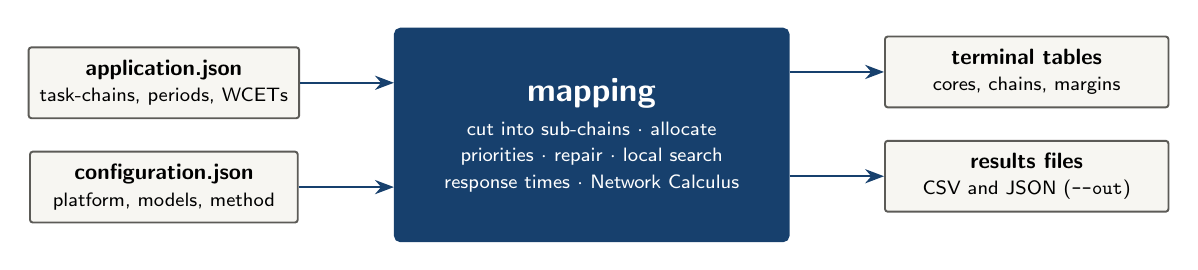
\begin{tikzpicture}[node distance=5mm]
\node[file,minimum width=34mm] (app) {\textbf{application.json}\\
	{\scriptsize task-chains, periods, WCETs}};
\node[file,minimum width=34mm,below=4mm of app] (cfg)
	{\textbf{configuration.json}\\{\scriptsize platform, models, method}};
\node[box,right=12mm of $(app.east)!0.5!(cfg.east)$,minimum width=50mm,
	minimum height=27mm,fill=brand,text=white,draw=brand] (tool)
	{\large\textbf{mapping}\\[3pt]
	 \scriptsize cut into sub-chains $\cdot$ allocate\\
	 \scriptsize priorities $\cdot$ repair $\cdot$ local search\\
	 \scriptsize response times $\cdot$ Network Calculus};
\node[file,right=12mm of tool,minimum width=36mm,yshift=8mm] (term)
	{\textbf{terminal tables}\\{\scriptsize cores, chains, margins}};
\node[file,below=4mm of term,minimum width=36mm] (csv)
	{\textbf{results files}\\{\scriptsize CSV and JSON (\opt{out})}};
\draw[arrow] (app.east) -- (tool.west |- app.east);
\draw[arrow] (cfg.east) -- (tool.west |- cfg.east);
\draw[arrow] (tool.east |- term.west) -- (term.west);
\draw[arrow] (tool.east |- csv.west) -- (csv.west);
\end{tikzpicture}
\end{center}

\begin{center}
\begin{tabularx}{\textwidth}{@{}XXX@{}}
\textsf{\textbf{\color{brand}How many cores?}}\newline
per ECU, with a lower bound and the margin left (critical scaling factor)
&
\textsf{\textbf{\color{brand}On time?}}\newline
every task-chain: maximum reaction time against its deadline, why late
&
\textsf{\textbf{\color{brand}Which architecture?}}\newline
zonal, domain, hybrid or distributed; star, tree, ring or any backbone
\end{tabularx}
\end{center}

\newpage
{\small\tableofcontents}
\newpage

\section{What the tool does}
\label{sec:what}

A vehicle function is a \emph{task-chain}: a sensor is sampled, data flows
through a sequence of periodic tasks, and an actuator is commanded. A
modern electrical/electronic (E/E) platform runs hundreds of them on a few
powerful ECUs linked by a Time-Sensitive Networking (TSN) Ethernet
backbone. \cmd{mapping} takes such an application and such a platform,
and answers three questions with a worst-case analysis behind every
number:
\begin{enumerate}
\item \textbf{How many cores} does each ECU need? The tool reports the
cores used, a lower bound that no mapping can beat, and the cores it had
to add to the platform.
\item \textbf{Does every task-chain meet its deadline}, once its tasks are
spread over cores and ECUs? The tool bounds the response time of every
task (fixed-priority scheduling), the delay of every message (Network
Calculus for the TSN shapers) and the maximum reaction time of every
task-chain under logical execution time (LET) communication.
\item \textbf{How much margin is left?} The critical scaling factor says
how much every WCET may grow before a core misses a deadline; the sizing
option lowers the utilization cap until a target margin is reached; and
the fixed-hardware option checks whether a software update still fits the
platform frozen at the start of production.
\end{enumerate}
The method is the one of the paper \emph{System-level mapping of automotive applications onto zonal E/E architectures} (\cmd{paper/ifupauline2026-system-level-mapping-automotive.pdf}).
The paper explains \emph{why} it works; this manual explains \emph{how} to
use it. You need no knowledge of the code before \cref{sec:code}.

\paragraph{The programs.} The build produces six programs; the repository
also has five Python scripts.

\begin{center}\small\row
\begin{tabularx}{\textwidth}{@{}>{\raggedright\arraybackslash}p{40mm}X@{}}
\toprule\rowcolor{white}
program & what it is for \\
\midrule
\cmd{mapping} & map one application on one platform, from files or generated; print or write the results (\cref{sec:running,sec:output,sec:usecases}) \\
\cmd{experiment} & run an experiment of the paper: many design points on many applications, in parallel, to a CSV file (\cref{sec:experiments}) \\
\cmd{baselines} & the heuristic against simulated annealing and a genetic algorithm (\cref{sec:ex-baselines}) \\
\cmd{export\_instance} & write an instance for the exact solver, or check an allocation (\cref{sec:ex-exact}) \\
\cmd{net\_export} & write the flows of a mapping for the network simulator (\cref{sec:ex-netsim}) \\
\cmd{golden} & regenerate the reference results of the regression test (\cref{sec:validation}) \\
\cmd{exact/exact.py}, \cmd{gap.py} & exact allocation with OR-Tools, and the optimality-gap study \\
\cmd{tests/netsim/netsim.py} & frame-level simulation of the TSN network \\
\cmd{tests/syssim/syssim.py} & simulation of the whole system: cores, LET and network \\
\cmd{paper/make\_figures.py} & the figures of the paper from the CSV files \\
\bottomrule
\end{tabularx}
\end{center}

\paragraph{Words.} The tool, the files and the paper use the words of the
field (\cref{tab:words}). A few names in the code are older or shorter:
an ECU is a \emph{controller} in the C sources, a sub-chain a
\emph{fragment}, and the central computer of the built-in zonal platform
is called \cmd{PCU}.

\begin{table}[ht]
\centering\small\row
\caption{The words of the tool.}
\label{tab:words}
\begin{tabularx}{\textwidth}{@{}>{\raggedright\arraybackslash}p{37mm}>{\raggedright\arraybackslash}p{38mm}X@{}}
\toprule\rowcolor{white}
word & in the files and output & meaning \\
\midrule
ECU & \key{ecus}, \key{ecu} & electronic control unit: a computer of the platform \\
central computer & \key{"role": "central"} & ECU that runs most functions; free software goes there first \\
zone controller & \key{"role": "zone"} & ECU of a physical zone, wired to its sensors and actuators \\
domain controller & \key{"role": "domain"} & ECU of one vehicle domain (chassis, body, ADAS\dots) \\
core type & \key{big}, \key{little}, \key{mcu}, \key{lockstep} & application cores, energy-efficient cores, microcontroller cores, lock-step safety cores \\
reference core & \key{wcet\_us} & the WCETs of the application file are on a core of speed 100\,\% \\
task-chain & \key{chains} & sequence of tasks from a sensor to an actuator \\
sub-chain & \emph{chain.index}, ``fragment'' & run of consecutive tasks of one chain placed together on one core \\
utilization cap $\varphi$ & \key{utilization\_cap}, \opt{phi} & largest load of a core, its LET task included \\
sub-chain limit $\sigma$ & \key{sigma}, \opt{sigma} & largest utilization of a sub-chain when chains are cut \\
allocation rule & \key{allocation}, \opt{algorithm} & BFDU, WFDU, FFDU or CADU (\cref{sec:conf-method}) \\
LET & \key{"communication": "implicit"} & logical execution time: data cross cores only at fixed instants \\
maximum reaction time & ``reaction'' & longest time from an event to the actuation that accounts for it: compared with the deadline \\
critical scaling factor & ``scaling'' & largest factor on every WCET that keeps the cores schedulable \\
\bottomrule
\end{tabularx}
\end{table}

\section{Installation}
\label{sec:install}

\paragraph{Requirements.} A C11 compiler (GCC or Clang), CMake 3.10 or
later, and OpenMP (optional: experiments in parallel). For the scripts:
Python 3 with \cmd{numpy}, \cmd{matplotlib} and \cmd{ortools} (the exact
solver only). For the paper and this manual: a LaTeX distribution (on
Debian: \cmd{texlive-latex-extra texlive-science texlive-pictures
texlive-fonts-extra}).

\paragraph{Build and test.}
\begin{shell}
cmake -S . -B build\\
cmake -{}-build build -j\\
cd build \&\& ctest -{}-output-on-failure\\
pip install -r requirements.txt \quad\# numpy, matplotlib, ortools
\end{shell}
The programs are in \cmd{build/bin}. All tests must pass
(\cref{sec:validation}); the exact-solver test runs only if OR-Tools is
installed. A build with the address and undefined-behaviour sanitizers
checks the memory accesses of the C code:
\begin{shell}
cmake -S . -B build-san -DMP\_SANITIZE=ON -DCMAKE\_BUILD\_TYPE=Debug
\end{shell}

\needspace{10\baselineskip}
\paragraph{First runs.} Each command below takes well under a second.
\begin{shell}
build/bin/mapping \quad\# a generated application, built-in zonal platform\\
build/bin/mapping examples/uc1\_central\_sizing/application.json \textbackslash\\
\quad examples/uc1\_central\_sizing/configuration.json -{}-cores\\
build/bin/mapping -{}-example-config domain > domain.json \quad\# a template\\
build/bin/mapping -{}-config domain.json -{}-chains 120 -{}-out results-domain
\end{shell}
The first run generates 300 task-chains and compares the four allocation
rules on the built-in zonal platform. The second maps the 24 functions of
use case~1 (\cref{sec:uc1}) and prints every core and every task-chain.
The last two write a template configuration file and map a generated
application on it, the results going to the files of
\cref{sec:outfiles}.

\section{Concepts in ten minutes}
\label{sec:concepts}

\subsection{Task-chains, tasks and their timing}

A \textbf{task} is periodic: it is released every period $T$ (in
microseconds), runs for at most its worst-case execution time (WCET) $C$,
and must end before its next release (implicit deadline). The WCETs of the
application file are measured on a \emph{reference core} of speed
100\,\%; on a core of speed $s$\,\% a task takes $C \cdot 100/s$, times an
optional factor for the type of the core (a neural network may gain more
than the speed ratio on a big core). Its \textbf{utilization} is
$C/T$: the share of a core it uses.

A \textbf{task-chain} is a sequence of tasks, each one using the output of
the previous one. Its first task usually reads a sensor and its last one
commands an actuator: those tasks are \emph{bound} to the ECU the sensor or
the actuator is wired to. The other tasks are \emph{free}: the tool decides
where they run. Consecutive tasks with the same period form an
\emph{activation pattern}; when the period changes along the chain, the
next task reads the last value written, up to one of its periods later.

\begin{figure}[ht]
\centering
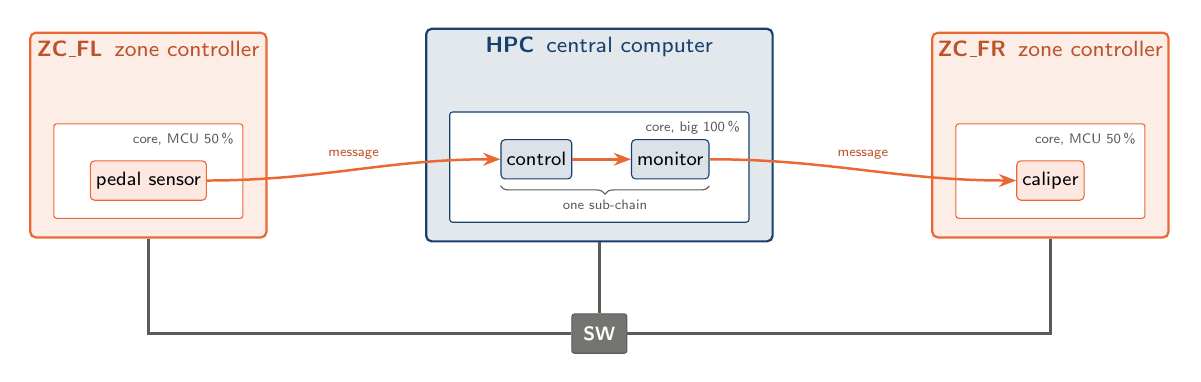
\begin{tikzpicture}[node distance=4mm]
% ECUs
\node[ecuzone,minimum width=30mm,minimum height=26mm] (fl) {};
\node[anchor=north,font=\sffamily\footnotesize\bfseries,text=accent!80!black]
	at (fl.north) {ZC\_FL\enspace\textmd{zone controller}};
\node[ecucentral,minimum width=44mm,minimum height=27mm,right=20mm of fl] (hpc) {};
\node[anchor=north,font=\sffamily\footnotesize\bfseries,text=brand]
	at (hpc.north) {HPC\enspace\textmd{central computer}};
\node[ecuzone,minimum width=30mm,minimum height=26mm,right=20mm of hpc] (fr) {};
\node[anchor=north,font=\sffamily\footnotesize\bfseries,text=accent!80!black]
	at (fr.north) {ZC\_FR\enspace\textmd{zone controller}};
% cores
\node[draw=accent,fill=white,rounded corners=1pt,minimum width=24mm,
	minimum height=12mm,anchor=south] (c1) at ([yshift=2.5mm]fl.south) {};
\node[anchor=north east,font=\sffamily\tiny,text=cmuted] at (c1.north east) {core, MCU 50\,\%};
\node[task=accent] (t0) at ([yshift=-1.2mm]c1.center) {pedal sensor};
\node[draw=brand,fill=white,rounded corners=1pt,minimum width=38mm,
	minimum height=14mm,anchor=south] (c2) at ([yshift=2.5mm]hpc.south) {};
\node[anchor=north east,font=\sffamily\tiny,text=cmuted] at (c2.north east) {core, big 100\,\%};
\node[task=brand] (t1) at ([xshift=-8mm,yshift=1.0mm]c2.center) {control};
\node[task=brand] (t2) at ([xshift=9mm,yshift=1.0mm]c2.center) {monitor};
\node[draw=accent,fill=white,rounded corners=1pt,minimum width=24mm,
	minimum height=12mm,anchor=south] (c3) at ([yshift=2.5mm]fr.south) {};
\node[anchor=north east,font=\sffamily\tiny,text=cmuted] at (c3.north east) {core, MCU 50\,\%};
\node[task=accent] (t3) at ([yshift=-1.2mm]c3.center) {caliper};
% switch and links
\node[switch,below=9mm of hpc] (sw) {SW};
\draw[link] (fl.south) |- (sw.west);
\draw[link] (hpc.south) -- (sw.north);
\draw[link] (fr.south) |- (sw.east);
% data flow
\draw[flow] (t0.east) to[out=0,in=180] node[above,font=\sffamily\tiny,text=accent!80!black]{message} (t1.west);
\draw[flow] (t1) -- (t2);
\draw[flow] (t2.east) to[out=0,in=180] node[above,font=\sffamily\tiny,text=accent!80!black]{message} (t3.west);
% sub-chain braces
\draw[decorate,decoration={brace,amplitude=3pt,mirror},cmuted]
	([yshift=-0.8mm]t1.south west) -- ([yshift=-0.8mm]t2.south east)
	node[midway,below=1.5pt,font=\sffamily\tiny,text=cmuted]{one sub-chain};
\end{tikzpicture}
\caption{A task-chain of four tasks on a zonal platform: the sensor task
is bound to the zone controller of the pedal, the actuator task to the one
of the caliper, the two free tasks form one sub-chain on a core of the
central computer. Two messages cross the network.}
\label{fig:chain}
\end{figure}

\subsection{Sub-chains, cores and the utilization cap}

The tool first cuts every task-chain into \textbf{sub-chains}: runs of
consecutive tasks that will share a core. It cuts where two tasks are bound
to different ECUs (\emph{forced cuts}), where they allow different ECUs or
core types, and wherever a sub-chain would exceed the \textbf{limit
$\sigma$} (a fraction of a core). Small sub-chains pack better; large ones
communicate less.

Every core runs its sub-chains and one \textbf{LET task}, at the highest
priority, that copies the data between cores. The load of a core is the
sum of the utilizations of its tasks and of its LET task; it may not exceed
the \textbf{utilization cap $\varphi$} (0.8 by default). A core is
\textbf{schedulable} when every task meets its deadline under fixed
priorities; the tool assigns the priorities with an optimal method
(Audsley's) restricted to the orders that respect the chain order.

\subsection{ECUs and their roles}

A platform is a list of ECUs, each with a \textbf{role}, its initial
cores (by type and speed), the type of core the tool may add, its memory
for the tasks and its largest number of cores.
\begin{itemize}
\item \key{central}: a central (vehicle) computer. Free sub-chains go to
the central computers first; the cores the tool adds for free sub-chains
are added there first. On a platform without a central computer, the ECUs
with the fastest cores play this part (the ADAS and infotainment
controllers of the domain template).
\item \key{zone}: a zone controller, wired to the sensors and actuators of
its area of the car.
\item \key{domain}: a domain controller (powertrain, chassis, ADAS\dots).
\item \key{ecu}: one ECU of a distributed architecture.
\end{itemize}
The generator of applications wires the sensors and actuators to every ECU
that is not a central computer; in an application file you bind each task
yourself.

\subsection{Communication: LET and the network}
\label{sec:concepts-let}

Two consecutive tasks on one core communicate through a register. Between
two cores, data cross only at the \textbf{LET instants} of the cores: the
LET task of the producer core copies the output out, and the LET task of
the consumer core reads it at the release of the consumer job
(\cref{fig:let}). Between two ECUs the copy also crosses the network. The
key \key{communication} of the \key{execution\_model} chooses when an
output is copied out:
\begin{itemize}
\item \key{implicit} (the default): at the first LET instant after the
producer ends, as in \cref{fig:let}. The delays are short, but they depend
on the response time of the producer.
\item \key{LET}: \textbf{strict LET}, at the end
of the period of the producer, whatever its response time. The data flow
is deterministic and the messages leave with almost no jitter, but every
crossing waits a full producer period. Option \texttt{-{}-strict-let}.
\end{itemize}

\begin{figure}[ht]
\centering
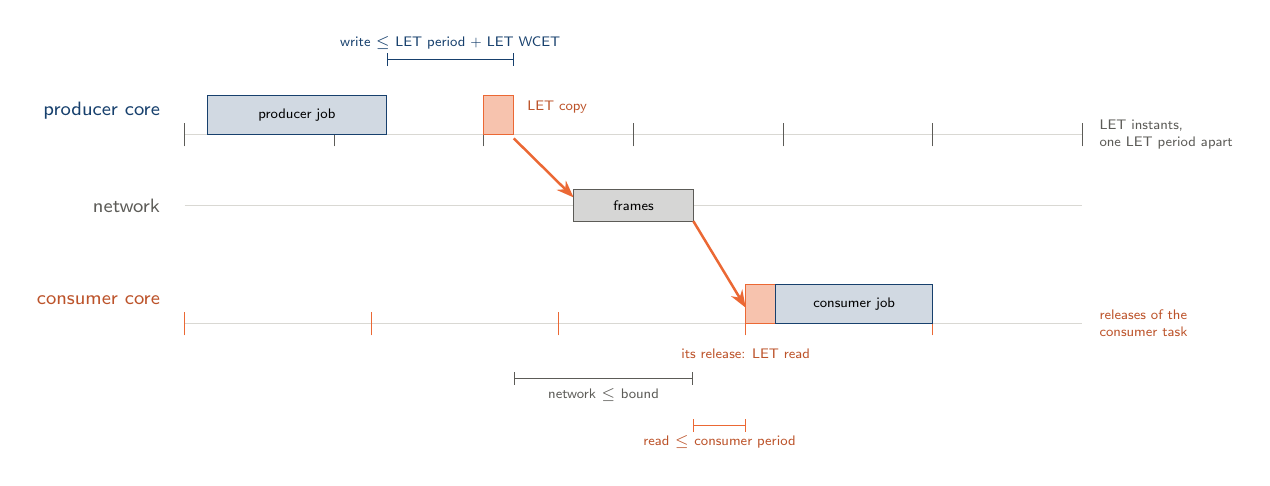
\begin{tikzpicture}[x=0.95mm,y=1mm]
% producer core
\node[anchor=east,font=\sffamily\scriptsize,text=brand] at (-2,20) {producer core};
\draw[cgrid] (0,17) -- (120,17);
\foreach \x in {0,20,...,120} \draw[cmuted] (\x,15.5) -- (\x,18.5);
\node[font=\sffamily\tiny,text=cmuted,anchor=west,align=left] at (121,17) {LET instants,\\one LET period apart};
\filldraw[draw=brand,fill=brand!20] (3,17) rectangle (27,22);
\node[font=\sffamily\tiny] at (15,19.5) {producer job};
\filldraw[draw=accent,fill=accent!40] (40,17) rectangle (44,22);
\node[font=\sffamily\tiny,anchor=west,text=accent!80!black] at (44.5,20.5) {LET copy};
% network
\node[anchor=east,font=\sffamily\scriptsize,text=cmuted] at (-2,8) {network};
\draw[cgrid] (0,8) -- (120,8);
\draw[flow] (44,16.5) -- (52,9);
\filldraw[draw=cmuted,fill=cmuted!25] (52,6) rectangle (68,10);
\node[font=\sffamily\tiny] at (60,8) {frames};
% consumer core
\node[anchor=east,font=\sffamily\scriptsize,text=accent!80!black] at (-2,-4) {consumer core};
\draw[cgrid] (0,-7) -- (120,-7);
\foreach \x in {0,25,...,100} \draw[accent] (\x,-8.5) -- (\x,-5.5);
\node[font=\sffamily\tiny,text=accent!80!black,anchor=west,align=left] at (121,-7) {releases of the\\consumer task};
\draw[flow] (68,6) -- (75,-5);
\filldraw[draw=accent,fill=accent!40] (75,-7) rectangle (79,-2);
\filldraw[draw=brand,fill=brand!20] (79,-7) rectangle (100,-2);
\node[font=\sffamily\tiny] at (89.5,-4.5) {consumer job};
\node[font=\sffamily\tiny,text=accent!80!black,anchor=north] at (75,-9) {its release: LET read};
% delays
\draw[|-|,brand] (27,26.5) -- (44,26.5) node[midway,above,font=\sffamily\tiny]{write $\le$ LET period + LET WCET};
\draw[|-|,cmuted] (44,-14) -- (68,-14) node[midway,below,font=\sffamily\tiny]{network $\le$ bound};
\draw[|-|,accent] (68,-20) -- (75,-20) node[midway,below,font=\sffamily\tiny,text=accent!80!black]{read $\le$ consumer period};
\end{tikzpicture}
\caption{One message between two cores, with implicit communication: the
output waits for the next LET instant of the producer core and for the
copy (with strict LET, for the end of the producer's period); it crosses
the network (between two ECUs); it is read at the next release of the
consumer. The analysis bounds each delay.}
\label{fig:let}
\end{figure}

The network is a switched Ethernet with the TSN mechanisms of IEEE 802.1:
credit-based shaping (\textbf{CBS}, 802.1Qav), time-aware shaping
(\textbf{TAS}, 802.1Qbv), asynchronous traffic shaping (\textbf{ATS},
802.1Qcr), frame preemption (802.1Qbu/802.3br) and frame replication and
elimination for reliability (\textbf{FRER}, 802.1CB). The messages are
grouped in one to three \emph{traffic classes} by the period of their
producer. Network Calculus bounds the delay of every message at every
output port of its route.

\subsection{What the analysis gives}
\label{sec:concepts-metrics}

\begin{itemize}
\item \textbf{Response time} of a task: the longest time from its release
to its end, with the interference of the higher-priority tasks of its core
(and of the shared memory, with the interference model).
\item \textbf{End-to-end response time} of a chain: the holistic sum of the
response times of its pattern runs and of the network bounds, without any
copy or sampling delay. It is a figure of merit, not a time of the system.
\item \textbf{End-to-end delay}: from the release of the job that samples
the sensor to the end of the first actuator job that uses the sample,
with every sampling and LET delay.
\item \textbf{Maximum reaction time}: the end-to-end delay plus one period
of the first task (an event waits at most that long to be sampled). It is
compared with the \textbf{deadline} of the chain. It also bounds the
maximum data age.
\item \textbf{Critical scaling factor}: the largest factor by which every
WCET of a core may be multiplied with its tasks still on time; the
smallest over the cores is the margin of the platform. It is below 1 when
a core misses a deadline.
\end{itemize}

\subsection{The method}
\label{sec:concepts-method}

\begin{figure}[ht]
\centering
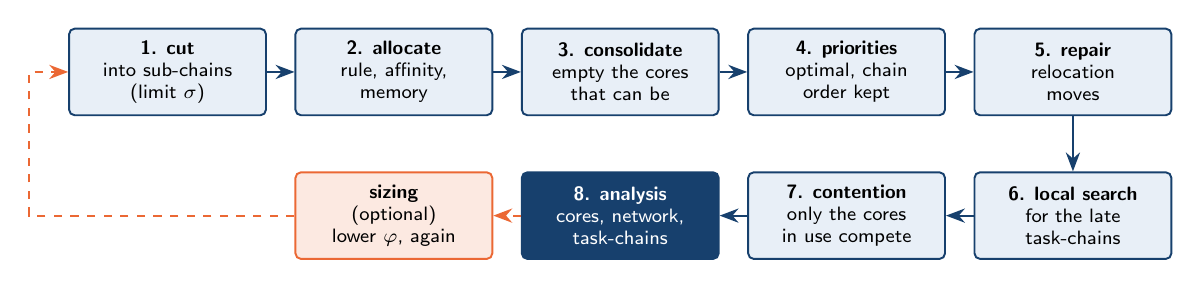
\begin{tikzpicture}[node distance=3.5mm,
	mstep/.style={box,minimum width=25mm,minimum height=11mm,font=\sffamily\scriptsize}]
\node[mstep] (p) {\textbf{1. cut}\\into sub-chains\\(limit $\sigma$)};
\node[mstep,right=of p] (a) {\textbf{2. allocate}\\rule, affinity,\\memory};
\node[mstep,right=of a] (c) {\textbf{3. consolidate}\\empty the cores\\that can be};
\node[mstep,right=of c] (s) {\textbf{4. priorities}\\optimal, chain\\order kept};
\node[mstep,right=of s] (r) {\textbf{5. repair}\\relocation\\moves};
\node[mstep,below=7mm of r] (l) {\textbf{6. local search}\\for the late\\task-chains};
\node[mstep,left=of l] (m) {\textbf{7. contention}\\only the cores\\in use compete};
\node[mstep,left=of m,fill=brand,text=white] (n) {\textbf{8. analysis}\\cores, network,\\task-chains};
\node[mstep,left=of n,draw=accent,fill=accentlight] (z) {\textbf{sizing}\\(optional)\\lower $\varphi$, again};
\draw[arrow] (p) -- (a); \draw[arrow] (a) -- (c); \draw[arrow] (c) -- (s);
\draw[arrow] (s) -- (r); \draw[arrow] (r) -- (l); \draw[arrow] (l) -- (m);
\draw[arrow] (m) -- (n);
\draw[arrow,accent,dashed] (n) -- (z);
\draw[arrow,accent,dashed] (z.west) -| ([xshift=-5mm]p.west) -- (p.west);
\end{tikzpicture}
\caption{The steps of one design point. With a target margin, the sizing
runs the steps again with a lower cap until the critical scaling factor
reaches the target.}
\label{fig:method}
\end{figure}

\Cref{fig:method} shows the steps of one \emph{design point} (one mapping
of one application with one set of parameters). Step~2 places the
sub-chains by decreasing utilization with one of four rules: best fit
(BFDU), worst fit (WFDU), first fit (FFDU) or communication aware (CADU,
fewest network hops created first); it tries first the cores that already
run part of the same chain (\emph{affinity}), and adds a core when no core
can take a sub-chain. Step~3 empties the cores whose sub-chains fit
elsewhere. Steps~5 and~6 move sub-chains to make every core schedulable
and to bring the late chains on time. The paper gives every step in
pseudo-code.

\section{The application file}
\label{sec:application}

The application file is a JSON object with an optional
\key{description} and a list of \key{chains}. Every chain has a list of
\key{tasks}, in chain order. Times are integers in microseconds; ECUs are
named as in the configuration file. The smallest file:

\begin{shell}
\{"chains": [\{"tasks": [\{"period\_us": 10000, "wcet\_us": 500\}]\}]\}
\end{shell}

A realistic chain, from the example of \opt{example-application}:
\begin{shell}
\{"name": "brake\_by\_wire", "deadline\_us": 10000, "tasks": [\\
\quad \{"name": "pedal\_sensor", "period\_us": 1000, "wcet\_us": 40,\\
\quad\ \ "ecu": "ZCU1", "message\_bytes": 16\},\\
\quad \{"name": "brake\_control", "period\_us": 1000, "wcet\_us": 120,\\
\quad\ \ "message\_bytes": 32\},\\
\quad \{"name": "caliper\_front\_left", "period\_us": 1000, "wcet\_us": 30,\\
\quad\ \ "ecu": "ZCU2"\}]\}
\end{shell}
The sensor task is bound to \cmd{ZCU1}, the actuator task to \cmd{ZCU2};
the control task is free. The chain must react within 10\,ms.

\begin{table}[ht]
\centering\small\row
\caption{The keys of a task-chain.}
\label{tab:chain-keys}
\begin{tabularx}{\textwidth}{@{}>{\raggedright\arraybackslash}p{30mm}>{\raggedright\arraybackslash}p{23mm}X@{}}
\toprule\rowcolor{white}
key & value & meaning \\
\midrule
\key{name} & text & shown in the outputs; at most 31 characters; distinct names (default: the chain number) \\
\key{deadline\_us} & integer & end-to-end deadline on the maximum reaction time; absent or 0: none \\
\key{ecu} & ECU name & the whole chain on that ECU (a local chain: every task bound there) \\
\key{ecus} & ECU names & the ECUs every task of the chain may run on \\
\key{replica\_group} & integer $>0$ & chains of one group are redundant copies: never on the same ECU (or core, \cref{sec:conf-method}); a group has at least two chains \\
\key{tasks} & list & the tasks, in chain order (mandatory) \\
\bottomrule
\end{tabularx}
\end{table}

\begin{table}[ht]
\centering\small\row
\caption{The keys of a task. Only the period and the WCET are mandatory.}
\label{tab:task-keys}
\begin{tabularx}{\textwidth}{@{}>{\raggedright\arraybackslash}p{35mm}>{\raggedright\arraybackslash}p{23mm}X@{}}
\toprule\rowcolor{white}
key & value & meaning \\
\midrule
\key{name} & text & shown in \cmd{mapping.csv}; at most 31 characters \\
\key{period\_us} & integer $\ge 1$ & period, also the deadline of the task \\
\key{wcet\_us} & integer $\ge 1$ & WCET on the reference core (speed 100\,\%), at most the period \\
\key{ecu} & ECU name & the task is bound there (its sensor or actuator) \\
\key{ecus} & ECU names & the ECUs it may run on (not with \key{ecu}) \\
\key{core\_types} & list & the core types it may run on: \key{big}, \key{little}, \key{mcu}, \key{lockstep} (a safety task: \key{["lockstep"]}) \\
\key{wcet\_factor\_percent} & \{type: \%\} & WCET on a core of that type, in \% of the WCET at the same speed (e.g.\ \key{\{"big": 70\}}: 30\,\% faster than its speed ratio on big cores) \\
\key{memory\_kb} & integer & code and data, counted against the memory of its ECU \\
\key{message\_bytes} & integer & size of its output message (absent: one minimum-size frame) \\
\key{memory\_accesses} & integer & requests to the shared memory per job (interference model; absent: from the access density) \\
\key{colocate\_with\_next} & true/false & must share a core with the next task \\
\bottomrule
\end{tabularx}
\end{table}

\paragraph{Checks.} The file is checked strictly: an unknown key, a value
of the wrong type or out of range, an unknown ECU, a WCET above its
period, a task bound to another ECU than its chain, a replica group of one
chain or two chains with the same name are errors, reported with the file,
the line and the key:
\begin{shell}
app.json:14: chain brake, task pedal: no ECU called "ZCU9"
\end{shell}

\begin{tip}[Generated applications]
\cmd{mapping -{}-generate -{}-chains 200 -{}-seed 4 > app.json} writes a
generated application (the statistics of an industrial engine-management
software, see the appendix of the paper) for the platform of the
configuration given with \opt{config}; you can then edit it. The options
\opt{replicas}, \opt{zone-only}, \opt{colocate}, \opt{lockstep} and
\opt{type-variation} add constraints to the generated chains.
\end{tip}

\section{The configuration file}
\label{sec:configuration}

The configuration file describes the hardware and the way to map onto it.
It has an optional \key{description} and five sections, each optional:
what a section leaves out keeps the default value of
\cref{tab:platform-keys,tab:exec-keys,tab:interference-keys,tab:network-keys,tab:method-keys}.
Without a \key{platform} section the platform is the built-in zonal one.

\begin{center}
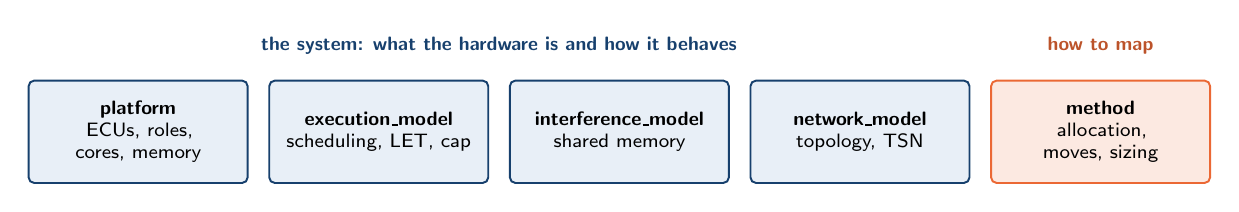
\begin{tikzpicture}[node distance=2.5mm,
	sec/.style={box,minimum width=27mm,minimum height=13mm,
		font=\sffamily\scriptsize,text width=25mm}]
\node[sec] (p) {\textbf{platform}\\ECUs, roles, cores, memory};
\node[sec,right=of p] (e) {\textbf{execution\_model}\\scheduling, LET, cap};
\node[sec,right=of e] (i) {\textbf{interference\_model}\\shared memory};
\node[sec,right=of i] (n) {\textbf{network\_model}\\topology, TSN};
\node[sec,right=of n,fill=accentlight,draw=accent] (m) {\textbf{method}\\allocation, moves, sizing};
\node[above=2mm of $(p.north west)!0.5!(n.north east)$,font=\sffamily\scriptsize\bfseries,text=brand]
	{the system: what the hardware is and how it behaves};
\node[above=2mm of m.north,font=\sffamily\scriptsize\bfseries,text=accent!80!black]
	{how to map};
\end{tikzpicture}
\end{center}

\begin{tip}[Start from a template]
\cmd{mapping -{}-example-config T} prints a complete configuration file,
every key with its value, for the template \cmd{T}: \cmd{zonal} (the
built-in platform), \cmd{domain}, \cmd{hybrid} or \cmd{distributed}
(\cref{fig:templates}). \cmd{mapping -{}-config FILE -{}-print-config} prints
the configuration in effect, options included: the way to check what the
tool understood.
\end{tip}

\subsection{\texttt{platform}: the ECUs}
\label{sec:conf-platform}

\key{"platform": \{"ecus": [...]\}} lists 1 to 32 ECUs. The ECU order sets
the numbering of the cores (central computers first, then one core of each
ECU of a role at a time) and the order in which ECUs receive new cores.

\begin{shell}
\{"name": "HPC", "role": "central",\\
\ "cores": [\{"type": "big", "count": 4, "speed\_percent": 100\},\\
\ \ \ \ \ \ \ \ \ \ \{"type": "little", "count": 4, "speed\_percent": 40\}],\\
\ "added\_core\_type": "big", "memory\_kb": 524288, "max\_cores": 12\}
\end{shell}

\begin{table}[ht]
\centering\small\row
\caption{The keys of an ECU (\key{platform.ecus}).}
\label{tab:platform-keys}
\begin{tabularx}{\textwidth}{@{}>{\raggedright\arraybackslash}p{30mm}>{\raggedright\arraybackslash}p{26mm}X@{}}
\toprule\rowcolor{white}
key & default & meaning \\
\midrule
\key{name} & (mandatory) & at most 31 characters, distinct \\
\key{role} & (mandatory) & \key{central}, \key{domain}, \key{zone} or \key{ecu} (\cref{sec:concepts}) \\
\key{cores} & (mandatory) & one group per core type: \key{type} (\key{big}, \key{little}, \key{mcu}, \key{lockstep}), \key{count} (initial cores, may be 0) and \key{speed\_percent} (of the reference core). A type without a group does not exist on this ECU \\
\key{added\_core\_type} & the first type & type of the cores the tool adds to this ECU (it adds a core of another type of the ECU when a sub-chain may only run there) \\
\key{memory\_kb} & 0 (unlimited) & memory for the code and data of the tasks \\
\key{max\_cores} & 0 (unlimited) & largest number of cores: a fixed hardware variant \\
\bottomrule
\end{tabularx}
\end{table}

\begin{figure}[p]
\centering
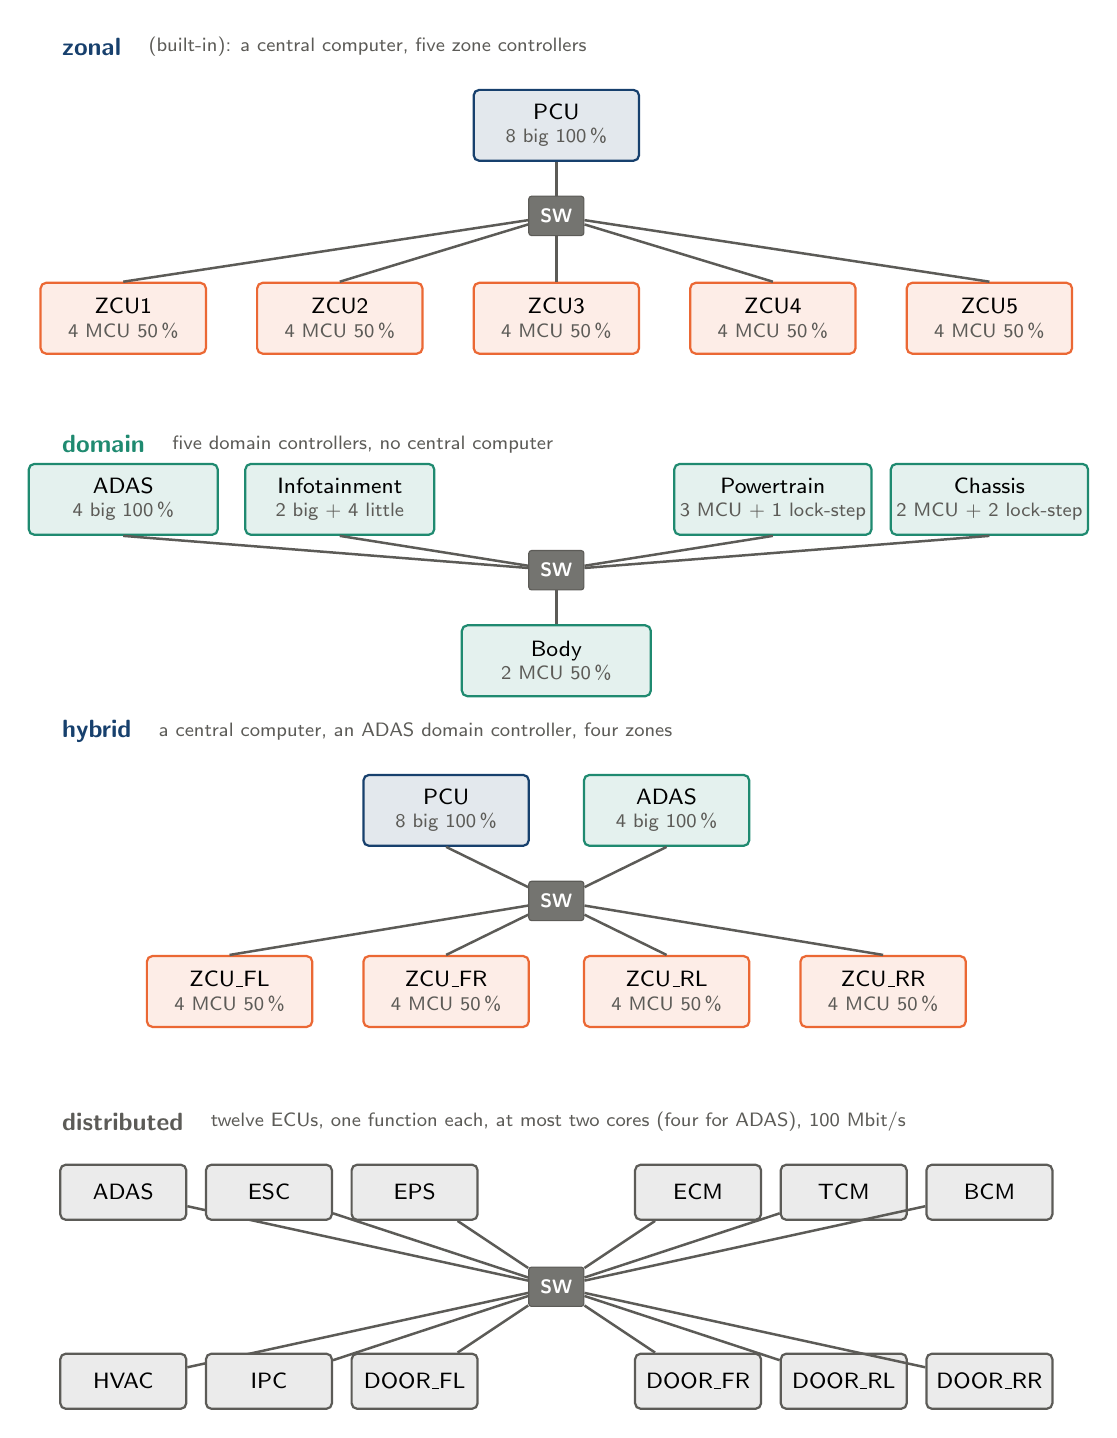
\begin{tikzpicture}[node distance=3mm]
% ---- zonal
\node[font=\sffamily\small\bfseries,text=brand,anchor=west] (tz) at (0,0.55) {zonal};
\node[font=\sffamily\scriptsize,text=cmuted,anchor=west] at ([xshift=1mm]tz.east) {(built-in): a central computer, five zone controllers};
\node[switch] (zsw) at (6.4,-1.6) {SW};
\node[ecucentral,minimum width=21mm] (zpcu) at (6.4,-0.45) {PCU\cores{8 big 100\,\%}};
\foreach \i/\x in {1/0.9,2/3.65,3/6.4,4/9.15,5/11.9} {
	\node[ecuzone,minimum width=21mm] (zz\i) at (\x,-2.9) {ZCU\i\cores{4 MCU 50\,\%}};
	\draw[link] (zz\i.north) -- (zsw);
}
\draw[link] (zpcu) -- (zsw);
% ---- domain
\node[font=\sffamily\small\bfseries,text=teal,anchor=west] (td) at (0,-4.5) {domain};
\node[font=\sffamily\scriptsize,text=cmuted,anchor=west] at ([xshift=1mm]td.east) {five domain controllers, no central computer};
\node[switch] (dsw) at (6.4,-6.1) {SW};
\foreach \n/\c/\x/\y [count=\k] in {ADAS/4 big 100\,\%/0.9/-5.2,Infotainment/2 big + 4 little/3.65/-5.2,
	Powertrain/3 MCU + 1 lock-step/9.15/-5.2,Chassis/2 MCU + 2 lock-step/11.9/-5.2} {
	\node[ecudomain,minimum width=24mm] (dd\k) at (\x,\y) {\n\cores{\c}};
	\draw[link] (dd\k.south) -- (dsw);
}
\node[ecudomain,minimum width=24mm] (dBody) at (6.4,-7.25) {Body\cores{2 MCU 50\,\%}};
\draw[link] (dBody) -- (dsw);
% ---- hybrid
\node[font=\sffamily\small\bfseries,text=brand,anchor=west] (th) at (0,-8.15) {hybrid};
\node[font=\sffamily\scriptsize,text=cmuted,anchor=west] at ([xshift=1mm]th.east) {a central computer, an ADAS domain controller, four zones};
\node[switch] (hsw) at (6.4,-10.3) {SW};
\node[ecucentral,minimum width=21mm] (hpcu) at (5.0,-9.15) {PCU\cores{8 big 100\,\%}};
\node[ecudomain,minimum width=21mm] (hadas) at (7.8,-9.15) {ADAS\cores{4 big 100\,\%}};
\draw[link] (hpcu.south) -- (hsw); \draw[link] (hadas.south) -- (hsw);
\foreach \n/\x [count=\k] in {ZCU\_FL/2.25,ZCU\_FR/5.0,ZCU\_RL/7.8,ZCU\_RR/10.55} {
	\node[ecuzone,minimum width=21mm] (hz\k) at (\x,-11.45) {\n\cores{4 MCU 50\,\%}};
	\draw[link] (hz\k.north) -- (hsw);
}
% ---- distributed
\node[font=\sffamily\small\bfseries,text=cmuted,anchor=west] (tdi) at (0,-13.1) {distributed};
\node[font=\sffamily\scriptsize,text=cmuted,anchor=west] at ([xshift=1mm]tdi.east) {twelve ECUs, one function each, at most two cores (four for ADAS), 100 Mbit/s};
\node[switch] (disw) at (6.4,-15.2) {SW};
\foreach \n/\x/\y in {ADAS/0.9/-14.0,ESC/2.75/-14.0,EPS/4.6/-14.0,ECM/8.2/-14.0,TCM/10.05/-14.0,BCM/11.9/-14.0,
	HVAC/0.9/-16.4,IPC/2.75/-16.4,DOOR\_FL/4.6/-16.4,DOOR\_FR/8.2/-16.4,DOOR\_RL/10.05/-16.4,DOOR\_RR/11.9/-16.4} {
	\node[ecuplain,minimum width=16mm,minimum height=7mm] (di) at (\x,\y) {\n};
	\draw[link] (di) -- (disw);
}
\end{tikzpicture}
\caption{The four templates of \opt{example-config}, star topology. The
zone, domain and distributed ECUs are wired to the sensors and actuators of
generated applications; ESC and EPS have one lock-step core each, ADAS two
big cores, the others one microcontroller core at 50\,\%.}
\label{fig:templates}
\end{figure}

\subsection{\texttt{execution\_model}: scheduling and communication}
\label{sec:conf-exec}

\begin{table}[ht]
\centering\small\row
\caption{The keys of \key{execution\_model}.}
\label{tab:exec-keys}
\begin{tabularx}{\textwidth}{@{}>{\raggedright\arraybackslash}p{36mm}>{\raggedright\arraybackslash}p{30mm}X@{}}
\toprule\rowcolor{white}
key & default & meaning \\
\midrule
\key{scheduling} & \key{fixed-priority preemptive} & the only one supported; written for the reader of the file \\
\key{communication} & \key{implicit} & between cores: \key{implicit} (an output is copied at the first LET instant after its producer ends) or \key{LET} (strict LET: published at the end of its producer's period) (\cref{sec:concepts-let}) \\
\key{utilization\_cap} & 0.8 & $\varphi$: largest load of a core, LET task included \\
\key{let\_task\_wcet\_us} & 50 & WCET of the LET task of a core that communicates, on the reference core \\
\key{wcet\_margin\_percent} & 0 & every WCET is raised by this percentage before the mapping \\
\bottomrule
\end{tabularx}
\end{table}

\subsection{\texttt{interference\_model}: shared-memory contention}
\label{sec:conf-interference}

The cores of one ECU share its memory; a request waits for the requests of
the other cores, served in round robin. A task then runs for its WCET plus
its requests times $(n-1)$ times the latency, $n$ the cores of the ECU that
run tasks; the tool iterates until the number of competing cores is the
one of the mapping.

\begin{table}[ht]
\centering\small\row
\caption{The keys of \key{interference\_model}.}
\label{tab:interference-keys}
\begin{tabularx}{\textwidth}{@{}>{\raggedright\arraybackslash}p{46mm}>{\raggedright\arraybackslash}p{24mm}X@{}}
\toprule\rowcolor{white}
key & default & meaning \\
\midrule
\key{shared\_memory\_arbitration} & \key{round-robin} & the only one supported \\
\key{memory\_latency\_ns} & 0 & time to serve one request; 0: no contention \\
\key{memory\_accesses\_per\_ms} & 1000 & requests per ms of reference WCET, for the tasks without \key{memory\_accesses} and for the LET tasks \\
\bottomrule
\end{tabularx}
\end{table}

\subsection{\texttt{network\_model}: the TSN backbone}
\label{sec:conf-network}

Every ECU has one full-duplex link to a switch. The \key{topology} gives
the switches: \key{star} (one switch), \key{tree} (one switch per ECU, all
linked to the switch of the root ECU), \key{ring} (one switch per ECU, in
ECU order) or \key{custom} (\cref{fig:topologies}). Routes are shortest
paths; the links of the central computers run at the backbone rate.

\begin{figure}[ht]
\centering
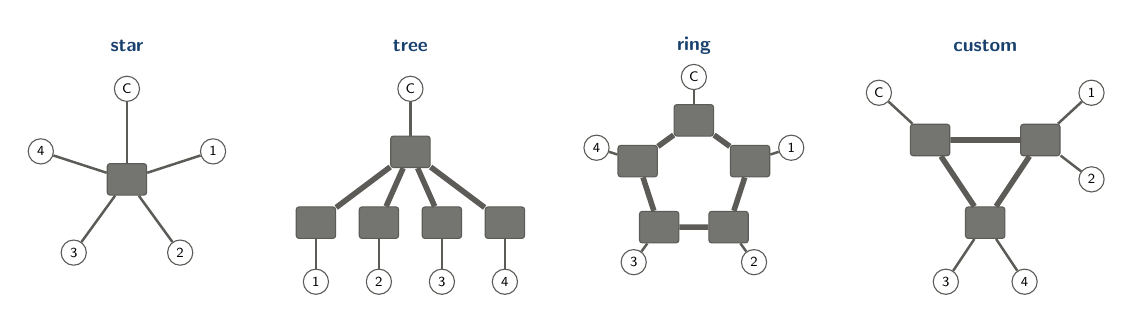
\begin{tikzpicture}[sw/.style={switch,minimum width=5mm,minimum height=4mm,font=\sffamily\tiny\bfseries},
	e/.style={draw=cmuted,fill=white,circle,inner sep=1.2pt,minimum size=3.2mm,font=\sffamily\tiny}]
% star
\begin{scope}
\node[font=\sffamily\scriptsize\bfseries,text=brand] at (0,1.7) {star};
\node[sw] (s) at (0,0) {};
\foreach \a/\n in {90/C,18/1,-54/2,-126/3,162/4} {
	\node[e] (e\n) at (\a:1.15) {\n}; \draw[link] (s) -- (e\n);}
\end{scope}
% tree
\begin{scope}[xshift=3.6cm]
\node[font=\sffamily\scriptsize\bfseries,text=brand] at (0,1.7) {tree};
\node[sw] (r) at (0,0.35) {};
\node[e] (rc) at (0,1.15) {C}; \draw[link] (r) -- (rc);
\foreach \x/\n in {-1.2/1,-0.4/2,0.4/3,1.2/4} {
	\node[sw] (t\n) at (\x,-0.55) {}; \draw[fast] (r) -- (t\n);
	\node[e] (te\n) at (\x,-1.3) {\n}; \draw[link] (t\n) -- (te\n);}
\end{scope}
% ring
\begin{scope}[xshift=7.2cm]
\node[font=\sffamily\scriptsize\bfseries,text=brand] at (0,1.7) {ring};
\foreach \a/\n in {90/C,18/1,-54/2,-126/3,162/4} {
	\node[sw] (q\n) at (\a:0.75) {};
	\node[e] (qe\n) at (\a:1.3) {\n}; \draw[link] (q\n) -- (qe\n);}
\draw[fast] (qC) -- (q1) -- (q2) -- (q3) -- (q4) -- (qC);
\end{scope}
% custom
\begin{scope}[xshift=10.9cm]
\node[font=\sffamily\scriptsize\bfseries,text=brand] at (0,1.7) {custom};
\node[sw] (u1) at (-0.7,0.5) {}; \node[sw] (u2) at (0.7,0.5) {};
\node[sw] (u3) at (0,-0.55) {};
\draw[fast] (u1) -- (u2) -- (u3) -- (u1);
\node[e] (ue1) at (-1.35,1.1) {C}; \draw[link] (u1) -- (ue1);
\node[e] (ue2) at (1.35,1.1) {1}; \draw[link] (u2) -- (ue2);
\node[e] (ue3) at (1.35,0.0) {2}; \draw[link] (u2) -- (ue3);
\node[e] (ue4) at (-0.5,-1.3) {3}; \draw[link] (u3) -- (ue4);
\node[e] (ue5) at (0.5,-1.3) {4}; \draw[link] (u3) -- (ue5);
\end{scope}
\end{tikzpicture}
\caption{The topologies, for a central computer C and four other ECUs:
the switches are dark, the backbone links thick. A custom topology may
have switches without ECUs and links of their own rates.}
\label{fig:topologies}
\end{figure}

A custom topology names its switches with the ECUs on each one, and the
links between switches (full duplex, at the backbone rate unless they
give theirs):
\begin{shell}
"topology": "custom",\\
"switches": [\{"name": "SW\_CENTRAL", "ecus": ["HPC"]\},\\
\ \ \ \ \ \ \ \ \ \ \ \ \{"name": "SW\_FRONT", "ecus": ["ADAS\_DC", "ZC\_FL", "ZC\_FR"]\},\\
\ \ \ \ \ \ \ \ \ \ \ \ \{"name": "SW\_REAR", "ecus": ["ZC\_RL", "ZC\_RR"]\}],\\
"switch\_links": [\{"from": "SW\_CENTRAL", "to": "SW\_FRONT", "mbps": 10000\},\\
\ \ \ \ \ \ \ \ \ \ \ \ \ \ \ \ \{"from": "SW\_CENTRAL", "to": "SW\_REAR", "mbps": 2500\},\\
\ \ \ \ \ \ \ \ \ \ \ \ \ \ \ \ \{"from": "SW\_FRONT", "to": "SW\_REAR"\}]
\end{shell}
The tool checks that every ECU is on one switch, that every switch can
reach every other one, and that no route is longer than 16 ports. With
FRER (ring or custom), the second route of a replicated message is the
shortest one that shares no link and no switch with the first between the
switch of the source and the switch of the destination.

\begin{table}[ht]
\centering\small\row
\caption{The keys of \key{network\_model}.}
\label{tab:network-keys}
\begin{tabularx}{\textwidth}{@{}>{\raggedright\arraybackslash}p{44mm}>{\raggedright\arraybackslash}p{24mm}X@{}}
\toprule\rowcolor{white}
key & default & meaning \\
\midrule
\key{standard} & \key{TSN} & the only one supported \\
\key{topology} & \key{star} & \key{star}, \key{tree}, \key{ring} or \key{custom} \\
\key{tree\_root} & first central & tree: the ECU whose switch is the root \\
\key{switches}, \key{switch\_links} & & custom topology only (above) \\
\key{link\_mbps} & 1000 & rate of the ECU links, Mbit/s \\
\key{backbone\_mbps} & link rate & rate of the links between switches and of the links of the central computers \\
\key{ecu\_link\_mbps} & & rates of single ECU links, e.g.\ \key{\{"HPC": 10000\}} \\
\key{switch\_latency\_us} & 2 & fabric and propagation delay per switch crossed \\
\key{link\_limit\_percent} & 100 & design limit of the LET load of a port; a port above it is overloaded \\
\key{traffic\_shaping} & \key{CBS} & \key{CBS}, \key{TAS} or \key{ATS} \\
\key{traffic\_classes} & 1 & 1 to 3 LET classes, by the period of their producer \\
\key{class\_max\_periods\_us} & 5000, 20000 & largest producer period of each class but the last (classes $-1$ values) \\
\key{idle\_slopes\_percent} & 75 (one class) & CBS: share of the port rate of each class \\
\key{proportional\_idle\_slopes} & true & CBS, several classes: the total of the shares divided at each port in proportion to the traffic of each class \\
\key{tas\_cycle\_us} & 500 & TAS: gate cycle \\
\key{tas\_windows\_percent} & 70 (one class) & TAS: window of each class, \% of the cycle \\
\key{frame\_preemption} & false & preemption of the best-effort frames \\
\key{frer} & false & ring or custom: messages of replicated chains over two disjoint routes \\
\bottomrule
\end{tabularx}
\end{table}

\subsection{\texttt{method}: how to map}
\label{sec:conf-method}

\begin{table}[ht]
\centering\small\row
\caption{The keys of \key{method}.}
\label{tab:method-keys}
\begin{tabularx}{\textwidth}{@{}>{\raggedright\arraybackslash}p{34mm}>{\raggedright\arraybackslash}p{18mm}X@{}}
\toprule\rowcolor{white}
key & default & meaning \\
\midrule
\key{allocation} & \key{FFDU} & BFDU (best fit: fullest core), WFDU (worst fit: emptiest core), FFDU (first fit), CADU (fewest network hops, then a central computer, then best fit); all by decreasing utilization \\
\key{sigma} & 0.4 & $\sigma$: largest utilization of a sub-chain, fraction of a reference core (at most the cap) \\
\key{affinity} & true & a sub-chain first tries the cores of the other sub-chains of its chain \\
\key{consolidation} & true & after the allocation, empty the cores whose sub-chains fit elsewhere (not with WFDU) \\
\key{swap\_moves} & false & also exchange sub-chains of two unschedulable cores, before the relocation moves (in the experiments it never repaired a core) \\
\key{relocation\_moves} & true & move sub-chains of unschedulable cores to schedulable ones \\
\key{local\_search} & true & move sub-chains to bring late task-chains on time \\
\key{replica\_separation} & \key{ecu} & replicas on different \key{ecu}s, or only on different \key{core}s \\
\key{fixed\_hardware} & false & add no core: a sub-chain that fits nowhere makes the mapping infeasible (software updates of a frozen platform) \\
\key{target\_scaling} & 0 (none) & sizing: lower the cap until the critical scaling factor reaches this value (e.g.\ 1.3) \\
\bottomrule
\end{tabularx}
\end{table}

\begin{warn}[Which rule?]
FFDU and BFDU give the fewest cores; CADU the fewest network messages, at
the price of more cores; WFDU spreads the load on every core, which is
wasteful at design time but good on hardware that is already paid for
(use case~4, \cref{sec:uc4}). \cmd{-{}-algorithm all} compares the four.
\end{warn}

\section{Running \texttt{mapping}}
\label{sec:running}

\begin{shell}
mapping [APPLICATION.json [CONFIGURATION.json]] [options]
\end{shell}

\begin{itemize}
\item \textbf{The application}: the file given first, or else an
application generated from \opt{seed} and \opt{chains} (or the small
detection chain with \opt{detection-chain}).
\item \textbf{The configuration}: the file given second (or with
\opt{config}), or else the built-in zonal platform and the default method.
\item \textbf{The rules}: without a configuration file the four allocation
rules are compared side by side; with one, the tool uses the rule of its
\key{method} section. \opt{algorithm A} chooses one rule, \opt{algorithm
all} the four.
\item \textbf{Options override the configuration file.} The options of the
built-in zonal platform (\opt{pcu-*}, \opt{zcu-*}, \opt{little-speed})
are refused when the file has its own \key{platform}: change the file
instead.
\end{itemize}

\begin{table}[ht]
\centering\small\row
\caption{The options of \cmd{mapping} (\cmd{mapping -{}-help}). The
configuration key each one overrides is in brackets.}
\label{tab:options}
\begin{tabularx}{\textwidth}{@{}>{\raggedright\arraybackslash}p{39mm}X@{}}
\toprule\rowcolor{white}
option & meaning \\
\midrule
\multicolumn{2}{@{}l}{\textsf{\textbf{\color{brand}files}}}\\
\opt{config FILE} & the configuration file (instead of the second argument) \\
\opt{example-config [T]} & print the template \cmd{zonal}, \cmd{domain}, \cmd{hybrid} or \cmd{distributed}, then exit \\
\opt{example-application} & print a small application file for the zonal platform, then exit \\
\opt{generate} & print the generated application as a file, then exit \\
\opt{print-config} & print the configuration in effect, options included, then exit \\
\opt{out DIR} & write the result files of \cref{sec:outfiles} into \cmd{DIR} \\
\multicolumn{2}{@{}l}{\textsf{\textbf{\color{brand}generated application}}}\\
\opt{seed N}, \opt{chains N} & seed (default \cmd{\$MP\_SEED} or 1) and number of task-chains (300) \\
\opt{detection-chain} & the detection chain: an illustrative chain of nine tasks \\
\opt{replicas P} & \% of the chains that are replicas of others (0) \\
\opt{colocate P} & \% of consecutive free tasks that must share a core (0) \\
\opt{zone-only P} & \% of chains whose free tasks avoid the central computers (0) \\
\opt{lockstep P} & \% of chains (safety) on lock-step cores only (0) \\
\opt{type-variation P} & WCET on each core type within $\pm P$\,\% of its speed ratio (0) \\
\multicolumn{2}{@{}l}{\textsf{\textbf{\color{brand}method}}}\\
\opt{algorithm A} & \cmd{BFDU}, \cmd{WFDU}, \cmd{FFDU}, \cmd{CADU} or \cmd{all} [\key{allocation}] \\
\opt{sigma S} & sub-chain limit, fraction of a core [\key{sigma}] \\
\opt{target-scaling F} & sizing for a critical scaling factor $F$ [\key{target\_scaling}] \\
\opt{no-affinity}, \opt{no-consolidation} & [\key{affinity}], [\key{consolidation}] off \\
\opt{no-relocation} & [\key{relocation\_moves}] off \\
\opt{swap} & [\key{swap\_moves}] on \\
\opt{no-repair} & no deadline-driven local search [\key{local\_search}] \\
\opt{fixed-hardware} & add no core [\key{fixed\_hardware}] \\
\opt{separate-cores} & replicas on different cores only [\key{replica\_separation}] \\
\multicolumn{2}{@{}l}{\textsf{\textbf{\color{brand}execution and interference models}}}\\
\opt{phi F} & utilization cap [\key{utilization\_cap}] \\
\opt{let C} & WCET of the LET tasks, \us{} [\key{let\_task\_wcet\_us}] \\
\opt{strict-let} & strict LET between cores instead of implicit communication [\key{communication}] \\
\opt{margin P} & WCET margin, \% [\key{wcet\_margin\_percent}] \\
\opt{memory-latency L} & ns per memory request [\key{memory\_latency\_ns}] \\
\opt{access-density N} & requests per ms of WCET [\key{memory\_accesses\_per\_ms}] \\
\multicolumn{2}{@{}l}{\textsf{\textbf{\color{brand}network model}}}\\
\opt{topology T} & \cmd{star}, \cmd{tree} or \cmd{ring} [\key{topology}] \\
\opt{link M}, \opt{backbone M} & rates, Mbit/s [\key{link\_mbps}, \key{backbone\_mbps}] \\
\opt{classes N} & 1 to 3 traffic classes, with their default boundaries and shares [\key{traffic\_classes}] \\
\opt{tas}, \opt{ats} & time-aware or asynchronous shaping [\key{traffic\_shaping}] \\
\opt{preemption}, \opt{frer} & [\key{frame\_preemption}], [\key{frer}] \\
\multicolumn{2}{@{}l}{\textsf{\textbf{\color{brand}built-in zonal platform only}}}\\
\opt{pcu-cores N}, \opt{pcu-speed P} & big cores of the central computer (8) and their speed (100\,\%) \\
\opt{pcu-little N}, \opt{little-speed P} & little cores of the central computer (0) and their speed (40\,\%) \\
\opt{zcu-cores N}, \opt{zcu-speed P} & cores of each zone controller (4) and their speed (50\,\%) \\
\opt{zcu-lockstep N} & lock-step cores of each zone controller (0) \\
\opt{pcu-memory K}, \opt{zcu-memory K} & memory for the tasks, KB (unlimited) \\
\multicolumn{2}{@{}l}{\textsf{\textbf{\color{brand}output}}}\\
\opt{cores} & also print every core and every task-chain \\
\bottomrule
\end{tabularx}
\end{table}

\paragraph{Exit status.} 0 when the tool ran (whether the mapping is
feasible or not), 1 on an internal error, 2 on an invalid option or file;
the error message gives the file, the line and the key.

\section{Reading the results}
\label{sec:output}

This section reads the output of use case~1 (\cref{sec:uc1}), produced by
\begin{shell}
mapping examples/uc1\_central\_sizing/application.json \textbackslash\\
\quad examples/uc1\_central\_sizing/configuration.json -{}-cores
\end{shell}

\subsection{What the tool understood}

The output starts with the application and the platform as the tool read
them: the number of task-chains and tasks, how many are bound to one ECU,
how many start with a sensor task and end with an actuator task, every ECU
with its cores, then the models and the method.

\listing[\fontsize{6.3pt}{7.6pt}\selectfont]{listings/uc1_input.txt}

\subsection{The summary table}
\label{sec:summary}

One column per allocation rule (here only FFDU, the rule of the file).

\begin{table}[h]
\centering\small\row
\caption{The rows of the summary table.}
\label{tab:summary-rows}
\begin{tabularx}{\textwidth}{@{}>{\raggedright\arraybackslash}p{50mm}X@{}}
\toprule\rowcolor{white}
row & meaning \\
\midrule
feasible & every sub-chain found a core; otherwise the line below the table says which one did not, and why (\cref{sec:infeasible}) \\
sub-chains, fragmentation rate, forced cuts & the partitioning: sub-chains, cuts in \% of the possible cuts, cuts between tasks bound to different ECUs \\
cores used $M$ & cores that run at least one task: \textbf{the sizing result}; then on central computers and on the other ECUs \\
lower bound on $M$ & no mapping of these sub-chains uses fewer cores (each ECU's bound load, and the total load, over the cap) \\
cores added, cores emptied & cores beyond the initial ones; cores emptied by the consolidation \\
schedulable cores SR & \% of cores where every task meets its deadline, after the priorities, the optional swaps, the relocations, and at the end \\
critical scaling factor & the margin of the platform (\cref{sec:concepts-metrics}); with sizing, the cap found and whether the target was reached \\
application / LET load, room left & in cores, summed over the cores used \\
task-chains schedulable / meeting deadline & \% of chains whose tasks are all schedulable; and also within their deadline over bounded routes \\
local search moves & moves kept by the deadline-driven local search \\
communications inside an ECU / inter-ECU & messages between two cores of one ECU (shared memory) and between ECUs (network flows) \\
replicated with FRER & flows sent over two routes \\
network delay bound, busiest port & the largest bound of a flow; the largest LET load of an output port \\
end-to-end response time, max reaction time & the largest values over the task-chains (\cref{sec:concepts-metrics}) \\
CPU time & time to compute the design point (and with the sizing) \\
\bottomrule
\end{tabularx}
\end{table}


\begin{minipage}[t]{0.47\textwidth}
\vspace{0pt}
\listingbox[\scriptsize]{listings/uc1_summary.txt}
\end{minipage}\hfill
\begin{minipage}[t]{0.5\textwidth}
\vspace{0pt}\small
\textbf{Partitioning.} 64 sub-chains for 73 tasks: most chains are cut
at both ends, where the sensor and the actuator are bound to zone
controllers (40 forced cuts).

\textbf{Cores.} 7 cores are used: 2 on the HPC and one in each zone
controller. The lower bound is 5: no mapping of these sub-chains can do
with fewer. No core was added; none had to be emptied.

\textbf{Schedulability.} Every core is schedulable after the priority
assignment; the relocation moves had nothing to do. The critical
scaling factor 1.302: every WCET may grow by 30\,\% before a core misses
a deadline.

\textbf{Load.} 2.70 cores of application load, 0.34 of LET copies, 2.56
cores left below the caps.

\textbf{Task-chains.} All on time; the local search kept 6 moves to get
there. 33 messages cross the network; the largest delay bound is
0.8\,ms on a port loaded at 0.5\,\%.

\textbf{Time.} The design point took less than a millisecond of CPU.
\end{minipage}


\subsection{Per ECU}

The second table gives, for every ECU and rule, the cores used, their
load in cores (LET included) and the smallest critical scaling factor of
its cores. Here \cmd{ZC\_FL} is the ECU with the least margin: its 1.302
is the factor of the platform.

\listing{listings/uc1_ecus.txt}

\subsection{Cores and task-chains}
\label{sec:cores-chains}

With \opt{cores}, a table per rule lists the cores in use: ECU, type and
speed, load and LET load (\% of the core), scaling factor,
schedulability, number of tasks, and the sub-chains on it as
\emph{chain.index}.

\listing[\tiny]{listings/uc1_cores.txt}

A second table follows every task-chain: its path as segments on cores,
with the indices of its sub-chains in brackets; the number of
communications inside an ECU and over the network; its maximum reaction
time and its deadline; and, if it is late, why: \emph{task late} (a task
misses its period), \emph{network} (a flow crosses an overloaded port) or
\emph{deadline} (the reaction time exceeds the deadline).

\listing[\fontsize{4.6pt}{5.6pt}\selectfont]{listings/uc1_chains.txt}

\begin{tip}[Reading a path]
\cmd{c6@ZC\_C(0) > c0@HPC(1) > c4@ZC\_RL(2)} (stability control) means:
sub-chain 0 runs on core c6 of zone controller \cmd{ZC\_C}, sub-chain 1
on core c0 of the HPC, sub-chain 2 on core c4 of \cmd{ZC\_RL}. The two
arrows are two inter-ECU communications, each costing LET delays and a
network transfer: 27\,ms of reaction time for tasks of 5\,ms.
\end{tip}

\subsection{When the mapping is infeasible}
\label{sec:infeasible}

A mapping is infeasible when a sub-chain fits on no core. The tool names
it and says why:
\begin{shell}
FFDU: infeasible, sub-chain 23.0 (0.8 \% of a reference core, 6144 KB,\\
free): not enough memory, at most 5120 KB left on the ECUs it may run on
\end{shell}
The other reasons are: no core of the ECUs it may run on has a type it
allows; the hardware is fixed (\opt{fixed-hardware}); the ECUs with memory
left already have their largest number of cores; or the sub-chain is
larger than an empty core (lower \opt{sigma}, or use faster cores).

\subsection{The result files}
\label{sec:outfiles}

\opt{out DIR} writes six files, one row per rule and item, so that a
spreadsheet or a script can take over.

\begin{table}[ht]
\centering\small\row
\caption{The files of \opt{out}.}
\label{tab:outfiles}
\begin{tabularx}{\textwidth}{@{}>{\raggedright\arraybackslash}p{24mm}X@{}}
\toprule\rowcolor{white}
file & content \\
\midrule
\cmd{summary.json} & one object per rule: the rows of the summary table, as numbers \\
\cmd{ecus.csv} & per rule and ECU: role, cores used, application and LET load (cores), critical scaling factor, memory used and capacity (KB), load of its egress and ingress network ports (\%) \\
\cmd{cores.csv} & per rule and core in use: ECU, type, speed, added or initial, load and LET load (\%), schedulable, critical scaling factor, tasks \\
\cmd{chains.csv} & per rule and task-chain: tasks, utilization, sub-chains, communications over the network and inside an ECU, end-to-end response time, maximum reaction time (both empty when the chain has no bound: a task above its period or an unbounded port), deadline, schedulable, network bounded, on time, why late \\
\cmd{mapping.csv} & per rule and task: chain and task (numbers and names), sub-chain, core, ECU, core type, priority, period, WCET on its core, response time (empty for a task above its period, which has none) \\
\cmd{system.json} & the timing model of each mapping (cores with their LET task and tasks, chains with the core of each task and the bound of each hop), for the full-system simulation (\cref{sec:ex-syssim}) \\
\bottomrule
\end{tabularx}
\end{table}

\section{Five use cases}
\label{sec:usecases}

Each use case is a realistic question, with its application and
configuration files in \cmd{examples/}. Together they use every key of the
two files. Run them from the root of the repository; the outputs below
come from these exact commands.

\begin{center}\small\row
\begin{tabularx}{\textwidth}{@{}>{\raggedright\arraybackslash}p{45mm}X@{}}
\toprule\rowcolor{white}
use case & what it shows \\
\midrule
1.\ sizing the central computer & a zonal platform, 24 vehicle functions; read every output; compare the rules; size for a margin \\
2.\ a fail-operational chassis & redundant task-chains, lock-step cores, a ring with frame replication (FRER), CADU \\
3.\ camera streams and control loops & a tree backbone, three traffic classes, TAS, ATS, frame preemption, link rates \\
4.\ software updates & sizing at the SOP, then updates on frozen hardware; why spreading the load helps then \\
5.\ a hybrid platform & big.LITTLE central computer, a domain controller, shared-memory contention, a custom backbone \\
\bottomrule
\end{tabularx}
\end{center}

% ---------------------------------------------------------------------------
\subsection{Use case 1: how many cores does the central computer need?}
\label{sec:uc1}

\paragraph{The question.} A carmaker moves 24 functions of chassis,
powertrain, ADAS, body and comfort onto a zonal platform: a
high-performance computer (HPC) and five zone controllers. The zone
controllers are chosen (two microcontroller cores at half the speed of the
reference core, 4\,MB for the tasks); the HPC variant is open. How many
cores must it have, and is every function on time?

\begin{figure}[ht]
\centering
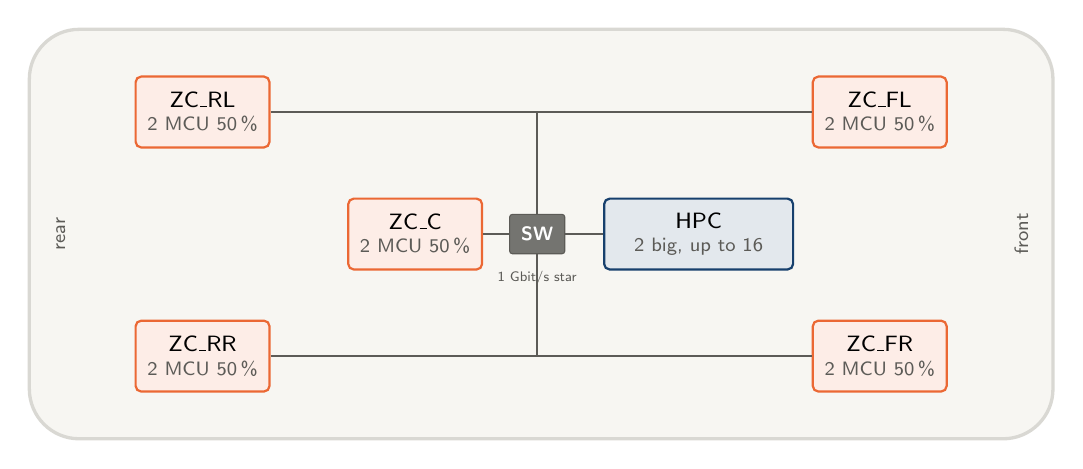
\begin{tikzpicture}
\draw[cgrid,line width=1.2pt,rounded corners=18pt,fill=cpaper] (0,0) rectangle (13,5.2);
\node[font=\sffamily\scriptsize,text=cmuted,rotate=90] at (12.6,2.6) {front};
\node[font=\sffamily\scriptsize,text=cmuted,rotate=90] at (0.4,2.6) {rear};
\node[ecuzone] (fl) at (10.8,4.15) {ZC\_FL\cores{2 MCU 50\,\%}};
\node[ecuzone] (fr) at (10.8,1.05) {ZC\_FR\cores{2 MCU 50\,\%}};
\node[ecuzone] (rl) at (2.2,4.15) {ZC\_RL\cores{2 MCU 50\,\%}};
\node[ecuzone] (rr) at (2.2,1.05) {ZC\_RR\cores{2 MCU 50\,\%}};
\node[ecuzone] (c) at (4.9,2.6) {ZC\_C\cores{2 MCU 50\,\%}};
\node[ecucentral,minimum width=24mm] (hpc) at (8.5,2.6) {HPC\cores{2 big, up to 16}};
\node[switch] (sw) at (6.45,2.6) {SW};
\draw[link] (fl) -| (sw); \draw[link] (fr) -| (sw);
\draw[link] (rl) -| (sw); \draw[link] (rr) -| (sw);
\draw[link] (c) -- (sw); \draw[link] (hpc) -- (sw);
\node[font=\sffamily\tiny,text=cmuted,anchor=north] at (6.45,2.25) {1 Gbit/s star};
\end{tikzpicture}
\caption{Use case 1: the platform, seen from above (front on the right).
Each zone controller has 4\,MB and at most 4 cores; the HPC 64\,MB and at
most 16 cores.}
\label{fig:uc1}
\end{figure}

\paragraph{The files.} \cmd{examples/uc1\_central\_sizing/}: the
configuration lists the six ECUs; the HPC starts with only 2 big cores,
so that the tool adds the cores it needs (\key{max\_cores} 16). The
application has 24 task-chains and 73 tasks: brake-by-wire and
steer-by-wire at 1\,ms with 5\,ms deadlines, stability and propulsion
control at 5 and 10\,ms, ADAS perception at 40 to 100\,ms (big cores only,
up to 16\,MB), body and comfort functions at 20\,ms to 1\,s, and three
local chains (two window lifters, the seat heating) bound to one zone
controller each.

\paragraph{Run.}
\begin{shell}
mapping examples/uc1\_central\_sizing/application.json \textbackslash\\
\quad examples/uc1\_central\_sizing/configuration.json -{}-cores
\end{shell}
\Cref{sec:output} reads this output line by line. The answer: \textbf{two
HPC cores suffice} (7 cores in all, the lower bound being 5), every core
is schedulable with a margin of 30\,\% on every WCET, and all 24 functions
meet their deadlines.

\paragraph{Compare the rules.} \cmd{-{}-algorithm all} maps with the four
rules:
\listing{listings/uc1_rules.txt}
CADU saves a core and a third of the network messages here, but one chain
misses its deadline; WFDU spreads the load over 12 cores and also leaves
one chain late. The largest maximum reaction time is about the same for
all rules: it is the chain of the tire pressure monitor, whose tasks run
once a second and whose deadline is 3\,s.

\paragraph{Size for a margin.} A margin of 30\,\% on every WCET is
little at the start of a project. \opt{target-scaling} lowers the
utilization cap until the critical scaling factor reaches the target:
\listing{listings/uc1_sizing.txt}
The cores are the same, but the load is spread so that every WCET may
grow by 68\,\% (target 1.5) or 100\,\% (target 2). The price is paid in
deadlines: with a lower cap, the control tasks of the 1\,ms by-wire chains
no longer fit the zone controller of their sensor and move to the HPC,
which adds two network hops. With the target 1.5 the steer-by-wire chain
is late, with the target 2 the two brake-by-wire chains too; the
\opt{cores} output names them.

% ---------------------------------------------------------------------------
\subsection{Use case 2: a fail-operational chassis}
\label{sec:uc2}

\paragraph{The question.} Steer-by-wire and brake-by-wire must survive
the failure of one ECU or one network link. Each is built as two
redundant task-chains (two \emph{lanes}) with their own sensors and
actuators; their safety monitors must run on lock-step cores; the
messages of the redundant chains are sent twice, over both directions of
an Ethernet ring (IEEE 802.1CB FRER). Is the platform of \cref{fig:uc2}
enough, and what does the redundancy cost on the network?

\begin{figure}[ht]
\centering
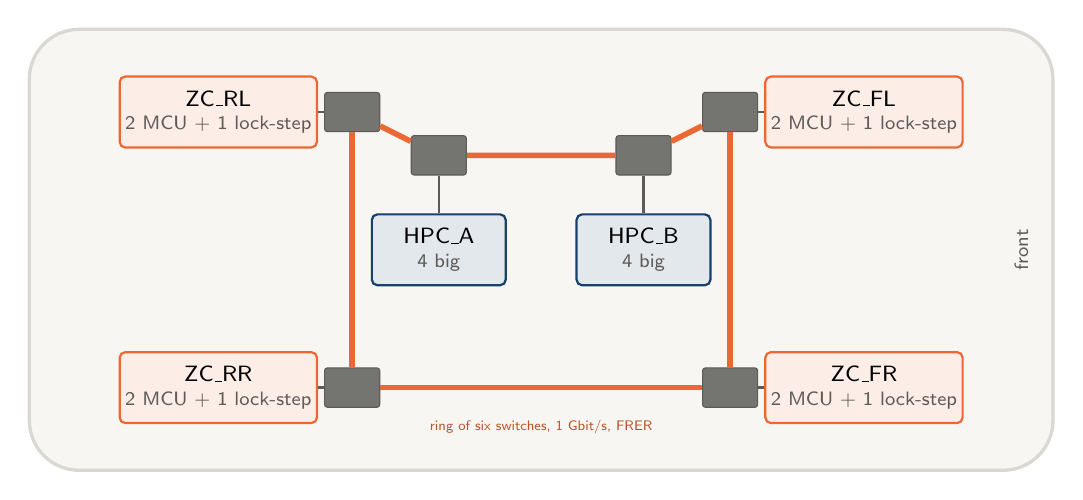
\begin{tikzpicture}
\draw[cgrid,line width=1.2pt,rounded corners=18pt,fill=cpaper] (0,0) rectangle (13,5.6);
\node[font=\sffamily\scriptsize,text=cmuted,rotate=90] at (12.6,2.8) {front};
\node[ecuzone] (fl) at (10.6,4.55) {ZC\_FL\cores{2 MCU + 1 lock-step}};
\node[ecuzone] (fr) at (10.6,1.05) {ZC\_FR\cores{2 MCU + 1 lock-step}};
\node[ecuzone] (rl) at (2.4,4.55) {ZC\_RL\cores{2 MCU + 1 lock-step}};
\node[ecuzone] (rr) at (2.4,1.05) {ZC\_RR\cores{2 MCU + 1 lock-step}};
\node[ecucentral] (a) at (5.2,2.8) {HPC\_A\cores{4 big}};
\node[ecucentral] (b) at (7.8,2.8) {HPC\_B\cores{4 big}};
\node[switch] (sa) at (5.2,4.0) {}; \node[switch] (sb) at (7.8,4.0) {};
\node[switch] (sfl) at (8.9,4.55) {}; \node[switch] (sfr) at (8.9,1.05) {};
\node[switch] (srl) at (4.1,4.55) {}; \node[switch] (srr) at (4.1,1.05) {};
\draw[link] (a) -- (sa); \draw[link] (b) -- (sb);
\draw[link] (fl) -- (sfl); \draw[link] (fr) -- (sfr);
\draw[link] (rl) -- (srl); \draw[link] (rr) -- (srr);
% ring in ECU order: A, B, FL, FR, RR, RL, A
\draw[fast,accent] (sa) -- (sb) -- (sfl);
\draw[fast,accent] (sfl) -- (sfr);
\draw[fast,accent] (sfr) -- (srr);
\draw[fast,accent] (srr) -- (srl);
\draw[fast,accent] (srl) -- (sa);
\node[font=\sffamily\tiny,text=accent!80!black] at (6.5,0.55) {ring of six switches, 1 Gbit/s, FRER};
\end{tikzpicture}
\caption{Use case 2: two central computers and four zone controllers with
lock-step cores, one switch per ECU, the switches in a ring in the order
of the configuration file.}
\label{fig:uc2}
\end{figure}

\paragraph{The files.} \cmd{examples/uc2\_redundant\_chassis/}. The
configuration sets a cap of 0.7 and a WCET margin of 10\,\% (safety
functions), a ring with FRER, two CBS classes (messages of tasks up to
5\,ms in the first one, with 50\,\% of the port, the others with 25\,\%),
and the CADU rule with replicas on different ECUs. In the application,
\key{replica\_group} 1 joins the two steering lanes and group 2 the two
braking lanes; the monitors have \key{"core\_types": ["lockstep"]} and the
ECUs they may use (\key{ecus}); the airbag is a local chain of the front
right zone on lock-step cores; the state estimator and the torque
vectoring of the vehicle dynamics share a core (\key{colocate\_with\_next});
the diagnostics may only run on the two HPCs (a chain-level \key{ecus}).

\paragraph{Run.}
\begin{shell}
mapping examples/uc2\_redundant\_chassis/application.json \textbackslash\\
\quad examples/uc2\_redundant\_chassis/configuration.json -{}-cores
\end{shell}
\listing[\fontsize{4.8pt}{5.8pt}\selectfont]{listings/uc2_chains.txt}
CADU keeps each lane in its own zones: the steering lanes never leave
\cmd{ZC\_FL} and \cmd{ZC\_FR} (one hop between two cores of the zone
controller, through its shared memory), so the replicas are on different
ECUs by construction, and only the braking lanes cross the ring: two
replicated flows. Every chain is on time with 8 cores.

\paragraph{The price of fewer messages.}
\listing{listings/uc2_rules.txt}
BFDU and FFDU need only 6 cores, but they send the control tasks of both
lanes to a central computer: twice as many messages, more than twice as
many replicated flows, and network bounds six times larger. With
\opt{separate-cores} the replicas may share an ECU (not a core): try it
to see which constraint costs what. A tree topology is refused with
\opt{frer}: a tree has no second route.

% ---------------------------------------------------------------------------
\subsection{Use case 3: camera streams and control loops on one backbone}
\label{sec:uc3}

\paragraph{The question.} Cameras (up to 120\,KB per frame), radars and a
lidar send their data from the zone controllers to the central computer,
while 1\,ms control loops cross the same switches between zones. Which
traffic shaping keeps the control loops on time, and what happens with a
slower link?

\begin{figure}[ht]
\centering
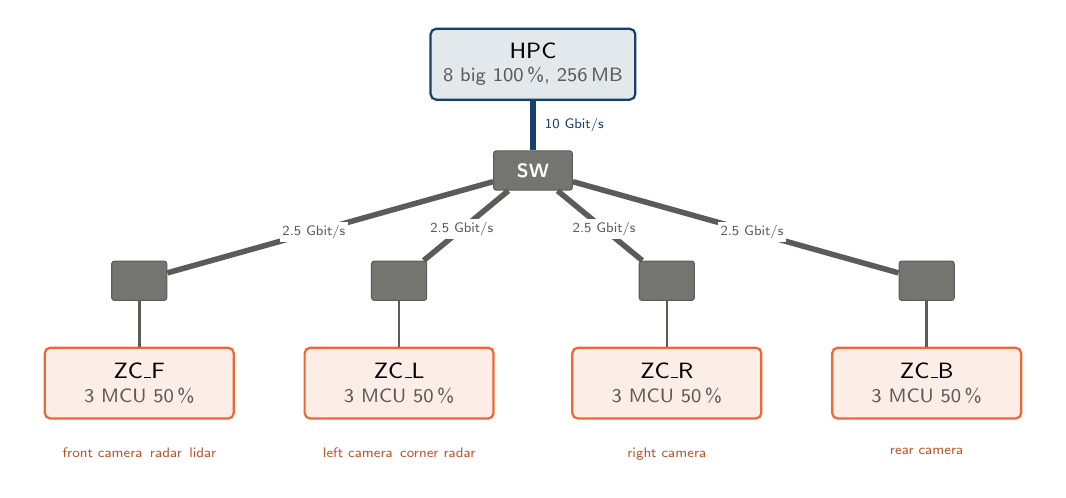
\begin{tikzpicture}
\node[switch,minimum width=10mm] (root) at (6.5,2.4) {SW};
\node[ecucentral,minimum width=26mm] (hpc) at (6.5,3.75) {HPC\cores{8 big 100\,\%, 256\,MB}};
\draw[fast,brand] (hpc) -- node[right,font=\sffamily\tiny,text=brand]{10 Gbit/s} (root);
\foreach \n/\x/\s [count=\k] in {ZC\_F/1.5/front camera\, radar\, lidar,ZC\_L/4.8/left camera\, corner radar,ZC\_R/8.2/right camera,ZC\_B/11.5/rear camera} {
	\node[switch] (s\k) at (\x,1.0) {};
	\draw[fast] (root) -- node[pos=0.55,font=\sffamily\tiny,text=cmuted,fill=white,inner sep=1pt]{2.5 Gbit/s} (s\k);
	\node[ecuzone,minimum width=24mm] (z\k) at (\x,-0.3) {\n\cores{3 MCU 50\,\%}};
	\draw[link] (s\k) -- (z\k);
	\node[font=\sffamily\tiny,text=accent!80!black,anchor=north,text width=26mm,align=center] at (\x,-1.0) {\s};
}
\end{tikzpicture}
\caption{Use case 3: a tree rooted at the switch of the HPC; the zone
links run at 1\,Gbit/s, the switches are linked at 2.5\,Gbit/s and the
HPC at 10\,Gbit/s.}
\label{fig:uc3}
\end{figure}

\paragraph{The files.} \cmd{examples/uc3\_tsn\_streams/}. The network
model is a \key{tree} with \key{tree\_root} \cmd{HPC},
\key{backbone\_mbps} 2500 and \key{ecu\_link\_mbps} 10000 for the HPC;
three traffic classes (producers up to 5\,ms, up to 40\,ms, the rest), TAS
with a cycle of 500\us{} and windows of 20, 40 and 20\,\%, frame
preemption, and a design limit of 80\,\% per port. The application has 12
chains: perception streams (40 to 100\,ms, messages of 3 to 120\,KB) and
control loops (1 to 20\,ms, messages of 8 to 32 bytes).

\paragraph{Run, then change the network.}
\begin{shell}
mapping examples/uc3\_tsn\_streams/application.json \textbackslash\\
\quad examples/uc3\_tsn\_streams/configuration.json [option]
\end{shell}
\listing{listings/uc3_network.txt}
With the file as it is, every chain is on time; the largest delay bound
(14\,ms) is the one of a camera frame of 120\,KB, sent through the TAS
window of its class. ATS (\opt{ats}) removes the waiting for the gates:
the largest bound falls to 2.9\,ms. With one class only
(\opt{classes 1}) the messages of the 1\,ms loops wait behind the camera
frames: the steering and braking loops miss their deadline, and so does
the front camera chain. With 100\,Mbit/s links
(\opt{link 100}) the ports carry 21\,\% of LET traffic and five chains are
late; ATS saves four of them.

% ---------------------------------------------------------------------------
\subsection{Use case 4: software updates on frozen hardware}
\label{sec:uc4}

\paragraph{The question.} The hardware of a car is fixed at the start of
production (SOP); its software keeps growing with updates for years. The
platform of use case~1 is sized at the SOP with a margin; then the HPC
variant is frozen. Do two later updates still fit, and how should they be
mapped?

\begin{figure}[ht]
\centering
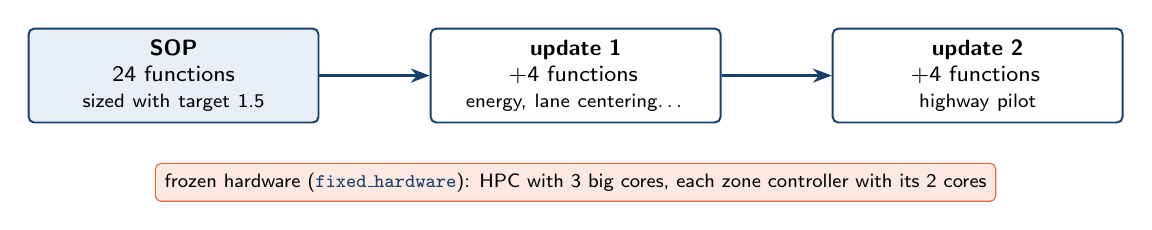
\begin{tikzpicture}[node distance=6mm]
\node[box,minimum width=36mm,text width=34mm] (sop) {\textbf{SOP}\\24 functions\\\scriptsize sized with target 1.5};
\node[box,right=14mm of sop,minimum width=36mm,text width=34mm,fill=white] (u1) {\textbf{update 1}\\+4 functions\\\scriptsize energy, lane centering\dots};
\node[box,right=14mm of u1,minimum width=36mm,text width=34mm,fill=white] (u2) {\textbf{update 2}\\+4 functions\\\scriptsize highway pilot};
\draw[arrow] (sop) -- (u1); \draw[arrow] (u1) -- (u2);
\node[draw=accent,fill=accentlight,rounded corners=2pt,below=5mm of u1,
	minimum width=104mm,font=\sffamily\scriptsize,align=center] (hw)
	{frozen hardware (\key{fixed\_hardware}): HPC with 3 big cores, each zone controller with its 2 cores};
\end{tikzpicture}
\caption{Use case 4: one platform, three versions of the software.}
\label{fig:uc4}
\end{figure}

\paragraph{The files.} \cmd{examples/uc4\_software\_updates/}:
\cmd{application\_sop.json} (the functions of use case~1),
\cmd{application\_update1.json} and \cmd{application\_update2.json} (four
more functions each, among them a highway pilot with 32\,MB of
perception); \cmd{configuration\_sop.json} (use case~1 with
\key{"target\_scaling": 1.5} and 512\,MB on the HPC) and
\cmd{configuration\_frozen.json} (the hardware chosen: 3 big cores on the
HPC, at most the initial cores everywhere, \key{"fixed\_hardware": true}).

\paragraph{Size at the SOP.}
\begin{shell}
mapping examples/uc4\_software\_updates/application\_sop.json \textbackslash\\
\quad examples/uc4\_software\_updates/configuration\_sop.json
\end{shell}
\listing{listings/uc4_sop.txt}
The SOP needs 2 HPC cores for a scaling factor of 1.68; the carmaker buys
a third one for the updates.

\paragraph{Map the updates on the frozen platform.} Each version is
mapped with the four rules on \cmd{configuration\_frozen.json}
(\cmd{-{}-algorithm all}); the table gives the task-chains on time:
\listing{listings/uc4_updates.txt}
Both updates fit the frozen hardware with every rule but CADU, which
cannot place a sensor task bound to \cmd{ZC\_FL} in update~2: no core of
that zone controller has room left, and the hardware is fixed. But the
rules that minimize the cores (BFDU, FFDU) now leave chains late:
packing the new functions moves the steering control off its zone
controller. \textbf{On frozen hardware the cores are already paid for}:
WFDU, which spreads the load over every core, keeps all chains of update~1
on time and 31 of 32 of update~2. The allocation objective changes after
the SOP.

% ---------------------------------------------------------------------------
\subsection{Use case 5: a hybrid platform with a big.LITTLE central computer}
\label{sec:uc5}

\paragraph{The question.} A hybrid platform keeps an ADAS domain
controller next to a central computer whose cores are of two types: 4
big and 4 little (at 40\,\% of the speed). The cores of each ECU share its
memory. Where does each function go, and how much does memory contention
cost?

\begin{figure}[ht]
\centering
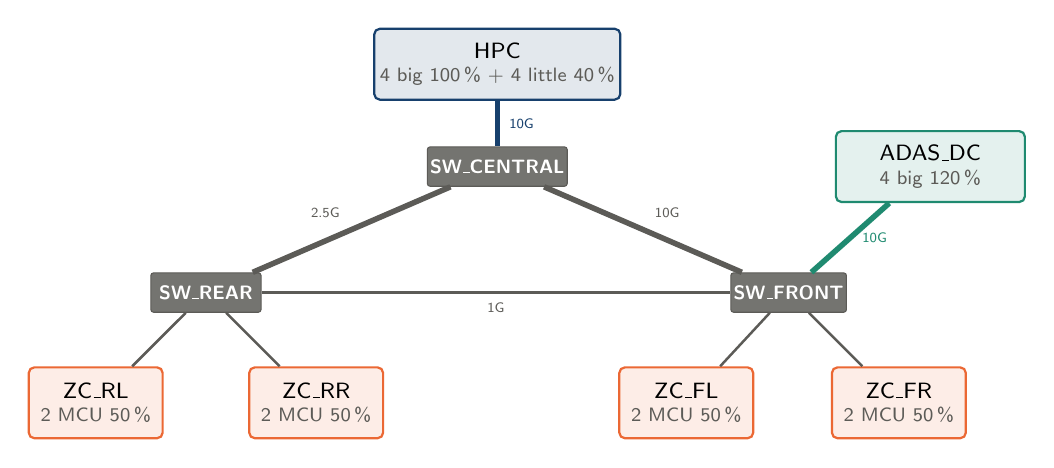
\begin{tikzpicture}
\node[switch,minimum width=16mm] (sc) at (6.5,2.6) {SW\_CENTRAL};
\node[switch,minimum width=14mm] (sf) at (10.2,1.0) {SW\_FRONT};
\node[switch,minimum width=14mm] (sr) at (2.8,1.0) {SW\_REAR};
\node[ecucentral,minimum width=30mm] (hpc) at (6.5,3.9) {HPC\cores{4 big 100\,\% + 4 little 40\,\%}};
\draw[fast,brand] (hpc) -- node[right,font=\sffamily\tiny,text=brand]{10G} (sc);
\draw[fast] (sc) -- node[above right,font=\sffamily\tiny,text=cmuted]{10G} (sf);
\draw[fast] (sc) -- node[above left,font=\sffamily\tiny,text=cmuted]{2.5G} (sr);
\draw[link] (sf) -- node[below,font=\sffamily\tiny,text=cmuted]{1G} (sr);
\node[ecudomain,minimum width=24mm] (adas) at (12.0,2.6) {ADAS\_DC\cores{4 big 120\,\%}};
\draw[fast,teal] (adas) -- node[right,font=\sffamily\tiny,text=teal]{10G} (sf);
\node[ecuzone] (fl) at (8.9,-0.4) {ZC\_FL\cores{2 MCU 50\,\%}};
\node[ecuzone] (fr) at (11.6,-0.4) {ZC\_FR\cores{2 MCU 50\,\%}};
\node[ecuzone] (rl) at (1.4,-0.4) {ZC\_RL\cores{2 MCU 50\,\%}};
\node[ecuzone] (rr) at (4.2,-0.4) {ZC\_RR\cores{2 MCU 50\,\%}};
\draw[link] (fl) -- (sf); \draw[link] (fr) -- (sf);
\draw[link] (rl) -- (sr); \draw[link] (rr) -- (sr);
\end{tikzpicture}
\caption{Use case 5: a custom backbone of three switches; the links of
the HPC and of the ADAS controller run at 10\,Gbit/s.}
\label{fig:uc5}
\end{figure}

\paragraph{The files.} \cmd{examples/uc5\_hybrid\_platform/}. The
configuration has every section: the platform (a \key{central}, a
\key{domain} and four \key{zone} ECUs, a 120\,\% ADAS controller), the
interference model (40\,ns per memory request), a \key{custom} topology
(\cref{sec:conf-network}), ATS with two classes, and CADU. In the
application the neural detector gains 30\,\% on big cores
(\key{"wcet\_factor\_percent": \{"big": 70\}}) and may only run on the ADAS
controller; the control laws lose less than the speed ratio on little
cores (\key{\{"little": 80\}}); the battery and comfort strategies may
only use little cores; every task gives its memory requests per job
(\key{memory\_accesses}).

\paragraph{Run.}
\begin{shell}
mapping examples/uc5\_hybrid\_platform/application.json \textbackslash\\
\quad examples/uc5\_hybrid\_platform/configuration.json -{}-cores
\end{shell}
\listing{listings/uc5_cores.txt}
The perception runs on the ADAS controller (core c8), the planning on a
big HPC core (c0), the strategies of battery, climate and body and the
diagnostics on one little HPC core (c4); the control loops stay in the
zone controllers. All chains are on time.

\paragraph{The cost of contention.} \opt{memory-latency} overrides the
interference model:
\listing{listings/uc5_contention.txt}
Without contention 6 cores suffice. At 40\,ns per request, the WCETs grow
with the number of cores competing for the memory of each ECU, and a
seventh core is needed; at 100\,ns an eighth one, and the application
load grows by 10\,\%. The tool finds the number of competing cores of
each ECU as a fixed point (more cores, more contention, longer WCETs).

\section{The experiments}
\label{sec:experiments}

The experiments of the paper are programs, not hand-made runs: anyone can
run them again and get the same files. This section explains, for each
one, the question it answers, what varies, what stays fixed, what it
measures and how to read its output.

\subsection{How an experiment runs}
\label{sec:ex-how}

\begin{figure}[ht]
\centering
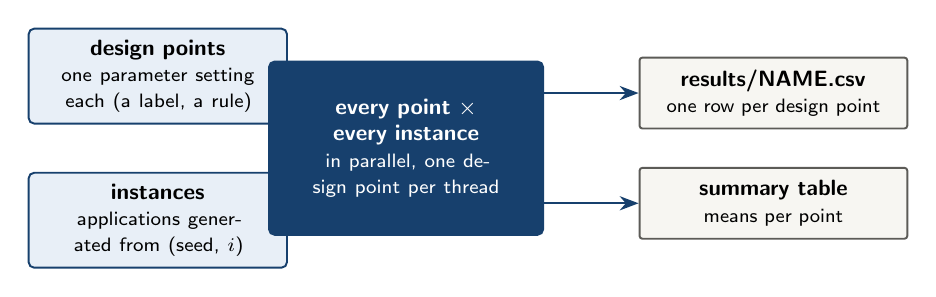
\begin{tikzpicture}[node distance=4mm]
\node[box,minimum width=32mm,text width=30mm] (pts) {\textbf{design points}\\\scriptsize one parameter setting each (a label, a rule)};
\node[box,minimum width=32mm,text width=30mm,below=6mm of pts] (inst) {\textbf{instances}\\\scriptsize applications generated from (seed, $i$)};
\node[box,right=14mm of $(pts)!0.5!(inst)$,minimum width=34mm,minimum height=22mm,
	fill=brand,text=white,text width=32mm] (run) {\textbf{every point $\times$ every instance}\\\scriptsize in parallel, one design point per thread};
\node[file,right=12mm of run,yshift=7mm,minimum width=34mm] (csv) {\textbf{results/NAME.csv}\\\scriptsize one row per design point};
\node[file,right=12mm of run,yshift=-7mm,minimum width=34mm] (tab) {\textbf{summary table}\\\scriptsize means per point};
\draw[arrow] (pts.east) -- (run.west |- pts.east);
\draw[arrow] (inst.east) -- (run.west |- inst.east);
\draw[arrow] (run.east |- csv.west) -- (csv.west);
\draw[arrow] (run.east |- tab.west) -- (tab.west);
\end{tikzpicture}
\caption{An experiment: every design point is run on the same generated
applications, so that two points differ only by their parameters.}
\label{fig:experiment}
\end{figure}

\begin{shell}
build/bin/experiment NAME [-{}-instances N] [-{}-jobs N] [-{}-seed N] [-{}-out FILE] [-{}-quiet]\\
build/bin/experiment all \quad\# every experiment, about three minutes on two cores
\end{shell}

An experiment is a list of \emph{design points}; each is run on several
generated applications (the \emph{instances}, 20 by default). Instance
$i$ always uses the application generated from (experiment seed, $i$):
every point sees the same applications, and the results do not depend on
the number of threads. Unless an experiment says otherwise, a point uses
the defaults: 300 task-chains of the default generator, the built-in
zonal platform (8 big cores on the PCU, 4 microcontroller cores at 50\,\%
on each of the five zone controllers), $\varphi = 0.8$, $\sigma = 0.4$,
LET tasks of 50\us, a star at 1\,Gbit/s with one CBS class, and every
step of the method.

The program prints a progress line, then a table with the means of the
metrics of the experiment over the instances of each point (over the
feasible ones for the mapping metrics), and writes every design point to
\cmd{results/NAME.csv} (\cref{sec:ex-csv}). The columns of the tables:

\begin{center}\small\row
\begin{tabularx}{\textwidth}{@{}>{\raggedright\arraybackslash}p{36mm}X@{}}
\toprule\rowcolor{white}
column & meaning (mean over the instances) \\
\midrule
feasible \% & instances where every sub-chain found a core \\
cores $M$, lower bound & cores used, and the lower bound on them \\
PCU, ZCU cores & cores used on the central computers, on the other ECUs \\
FR \% & fragmentation rate: cuts in \% of the possible cuts \\
SR sched, SR \% & schedulable cores after the priority assignment, and at the end \\
net hops, port max \% & inter-ECU communications; LET load of the busiest port \\
on time, misses & task-chains meeting their deadline (\%), late ones \\
reaction max & the largest maximum reaction time (ms) \\
scaling & critical scaling factor \\
CPU s & CPU time of a design point \\
\bottomrule
\end{tabularx}
\end{center}

\subsection{Experiments of the method}

\begin{experimentbox}{sweep}{the sub-chain limit against the rule}
\exitem{Question.} How does the limit $\sigma$ trade cores against
communications, and which rule packs best?
\exitem{Varies.} $\sigma \in \{0.02, 0.03, 0.05, 0.1, 0.2, 0.4, 0.8\}$
$\times$ the four rules: 28 points.
\exitem{Measures.} Cores and lower bound, cores per ECU kind, fragmentation
rate, schedulable cores, chains on time, maximum reaction time, CPU time.
\exitem{Reading.} A small $\sigma$ cuts chains into many small sub-chains:
fewer cores (they pack like sand), but more communications and longer
reaction times. Most chains use less than 8\,\% of a core, so the cuts
happen below $\sigma \approx 0.1$. WFDU uses every core of the platform
(28): it spreads on purpose.
\end{experimentbox}

\begin{experimentbox}{scaling}{CPU time against the size}
\exitem{Question.} Is the method fast enough for a whole vehicle?
\exitem{Varies.} 50 to 3200 task-chains (doubling) $\times$ the four rules;
2 instances per point.
\exitem{Measures.} Chains, tasks, feasibility, cores, schedulable cores,
CPU time of the placement phases and of the whole design point.
\exitem{Reading.} The CPU time grows a little faster than linearly: about
2\,s for 2000 chains on one core. The exact solver needs seconds to a
minute for 300 chains (\cref{sec:ex-exact}).
\end{experimentbox}

\begin{experimentbox}{architecture}{speed of the zone controllers}
\exitem{Question.} How fast must the zone controllers be?
\exitem{Varies.} Zone core speed 25, 50, 75, 100\,\% (PCU at 100\,\%)
$\times$ the four rules.
\exitem{Measures.} Cores (total, PCU, zones), lower bound, schedulable
cores, chains on time, LET load.
\exitem{Reading.} Slow zone cores take more cores for the tasks bound to
the zones; the free sub-chains go to the PCU anyway.
\end{experimentbox}

\begin{experimentbox}{affinity}{allocation with and without affinity}
\exitem{Question.} Does trying the cores of the other sub-chains of the
same chain first save communications?
\exitem{Varies.} $\sigma \in \{0.2, 0.4, 0.6\}$ $\times$ affinity on/off
$\times$ the four rules.
\exitem{Measures.} Cores, communications inside an ECU and over the
network, schedulable cores, chains on time, reaction time.
\exitem{Reading.} Compare each point with its twin without affinity: the
same cores, fewer hops.
\end{experimentbox}

\begin{experimentbox}{ablation}{each step of the method removed}
\exitem{Question.} What does each step of \cref{fig:method} bring?
\exitem{Varies.} Seven variants: the full method; without affinity;
without consolidation; with the optional swap moves; without relocation moves;
without the local search; without any of them (bin packing and the
priority assignment only), on two settings, \emph{default} and
\emph{stressed} (cores filled up to $\varphi = 1$, deadlines at 200\,\% of
the pattern periods instead of 300\,\%), $\times$ FFDU and CADU: 28
points.
\exitem{Measures.} Cores, schedulable cores after the priorities and at
the end, network hops, chains on time and late, CPU time.
\exitem{Reading.} Compare each variant with \emph{full}. With the default
setting, the consolidation saves cores (14.4 instead of 15.8 for FFDU) and
the local search brings chains on time (92.6 instead of 88.4\,\%). The
relocation moves only matter when cores are unschedulable, which happens
in the stressed setting (without them, 0.7\,\% of the cores stay
unschedulable). The swap moves change nothing, which is why they are off
by default.
\end{experimentbox}

\begin{experimentbox}{practice}{the method against practitioner rules}
\exitem{Question.} Does the method beat what an engineer would do by
hand?
\exitem{Varies.} The method with FFDU and with CADU; \emph{whole chains}
(cut only where the ECUs force it: $\sigma = \varphi$); \emph{central
only} (the free software on the central computer, the zones only for the
tasks bound there); both together; \emph{load balancing} (WFDU).
\exitem{Measures.} Cores (total, PCU, zones), lower bound, hops, busiest
port, chains on time, reaction time.
\exitem{Reading.} Keeping chains whole costs little here (the chains are
small), but see \cmd{limit}; putting all free software on the central
computer costs cores, network traffic and deadlines; load balancing uses
every core.
\end{experimentbox}

\begin{experimentbox}{limit}{the sub-chain limit where it matters}
\exitem{Question.} Why cut task-chains at all, and is the default
$\sigma = 0.4$ right?
\exitem{Varies.} $\sigma \in \{0.4, 0.6, 0.8\}$ (0.8 is the cap: whole
chains) on three settings: the default point, shared-memory contention at
50\,ns, and 600 task-chains; $\times$ FFDU and CADU: 18 points.
\exitem{Measures.} Feasibility, cores and lower bound, hops, chains on
time, CPU time.
\exitem{Reading.} At the default point a larger $\sigma$ changes little
(CADU saves about a core). With contention, the WCETs grow once the
sub-chains are placed, and a large sub-chain no longer fits any core:
only 45\,\% of the instances are feasible at $\sigma = 0.8$, 95\,\% at
0.6, all at 0.4. That is why the default is 0.4.
\end{experimentbox}

\begin{experimentbox}{deadlines}{deadlines and the local search}
\exitem{Question.} How tight can the deadlines be, and how much does the
local search recover?
\exitem{Varies.} Deadlines at 200, 300, 400, 600\,\% of the sum of the
pattern periods of each chain $\times$ local search on/off $\times$ the
four rules.
\exitem{Measures.} Cores, chains on time, late chains, moves kept, reaction
time, CPU time.
\end{experimentbox}

\begin{experimentbox}{fill}{the utilization cap}
\exitem{Question.} How high may the cores be filled?
\exitem{Varies.} $\varphi \in \{0.6, 0.7, 0.8, 0.9, 1.0\}$ $\times$ the four
rules.
\exitem{Measures.} Cores, schedulable cores after the priorities and at the
end, scaling factor, chains on time, CPU time of the placement.
\exitem{Reading.} Up to 0.9 the optimal priority assignment makes every
core schedulable; at 1.0 about 1\,\% of the cores are not (the periods are
not harmonic), and the relocation moves repair all of them.
\end{experimentbox}

\begin{experimentbox}{let}{the cost of the LET tasks}
\exitem{Varies.} WCET of the LET task: 10, 50, 100, 200\us{} $\times$ the
four rules.
\exitem{Measures.} Cores, LET load, communications on a core, schedulable
cores, chains on time.
\end{experimentbox}

\begin{experimentbox}{communication}{implicit communication or strict LET}
\exitem{Question.} What does the determinism of strict LET cost, against
implicit communication?
\exitem{Varies.} The two schemes on three settings: the default point,
deadlines at 500\,\%, and a ring with three classes; $\times$ FFDU and
CADU: 12 points.
\exitem{Measures.} Cores, hops, largest network bound, reaction times,
chains on time.
\exitem{Reading.} The cores do not change. Strict LET removes the response
time from the jitter of the flows, so the largest network bound falls by
15 to 19\,\%, but every crossing between cores waits for the end of the
producer's period: 30 points fewer chains on time with FFDU, 16 with CADU,
and only 4 and 1.5 with deadlines at 500\,\%.
\end{experimentbox}

\begin{experimentbox}{margins}{WCET margin or sizing}
\exitem{Question.} Two ways to keep a margin: raise every WCET at design
time, or size for a scaling factor. Which one costs fewer cores for the
same margin?
\exitem{Varies.} WCET margin 0, 10, 20, 40\,\%; then targets 1.10, 1.25,
1.50 for the sizing; $\times$ the four rules.
\exitem{Measures.} Cores, application load, schedulable cores, scaling
factor, cap found, target reached, chains on time.
\end{experimentbox}

\subsection{Experiments of the platform}

\begin{experimentbox}{cores}{types of cores}
\exitem{Question.} What do little cores and lock-step cores change?
\exitem{Varies.} Four platforms: PCU with 8 big cores or 4 big + 8 little;
zones with 4 microcontroller cores or 2 + 2 lock-step, the safety chains
(10\,\%) on lock-step cores only; every WCET up to 30\,\% off its speed
ratio on each type; $\times$ the four rules.
\exitem{Measures.} Cores (total, PCU, zones), application load, scaling
factor, chains on time.
\end{experimentbox}

\begin{experimentbox}{constraints}{spatial constraints}
\exitem{Varies.} None; 10, 20, 30\,\% of replicated chains (on other
ECUs); 20\,\% replicated on other cores only; 20\,\% of zone-only chains;
30\,\% of co-located tasks; 8\,MB of memory per zone controller; $\times$
the four rules.
\exitem{Measures.} Cores (total, PCU, zones), hops, chains on time,
reaction time.
\exitem{Reading.} Each constraint takes freedom from the allocation: its
price is read in cores and hops against the point \emph{none}.
\end{experimentbox}

\begin{experimentbox}{contention}{shared-memory contention}
\exitem{Varies.} Memory latency 0, 20, 50, 100\,ns per request (1000
requests per ms of WCET), $\times$ the four rules.
\exitem{Measures.} Cores (total, PCU, zones), application load, schedulable
cores, scaling factor, chains on time.
\exitem{Reading.} Contention grows with the cores used on an ECU, and more
load needs more cores: a packed mapping pays the most.
\end{experimentbox}

\begin{experimentbox}{dse}{four E/E architectures}
\exitem{Question.} For the same vehicle functions, which architecture
needs the fewest cores and the least network traffic, and up to what size
of software does each one work?
\exitem{Varies.} The four templates of \cref{fig:templates}
(distributed, domain, hybrid, zonal) $\times$ 100, 200, 300 task-chains
$\times$ FFDU and CADU: 24 points. The generator draws the same functions
for every template (the same seeds); their sensors and actuators are
wired to the ECUs that are not central computers.
\exitem{Measures.} Feasibility, cores and lower bound, hops, busiest port,
chains on time, reaction time, CPU time.
\exitem{Reading.} The distributed architecture runs out of cores as the
software grows (each small ECU has at most two cores, the ADAS controller
four): every instance is feasible at 100 chains, half of them with FFDU
at 300. The domain, hybrid and zonal ones all absorb 300 chains; the
hybrid and domain ones need about a core less than the zonal one, because
part of the bound work runs on big cores.
\end{experimentbox}

\begin{experimentbox}{lifecycle}{the SOP, then software updates}
\exitem{Question.} How many updates does a core bought at the SOP buy?
\exitem{Varies.} The cap at the SOP: 0.5, 0.6, 0.7, 0.8 $\times$ the four
rules. The platform is then fixed (the cores the SOP mapping uses), and
ten updates of 15 new task-chains each are mapped on it at $\varphi =
0.8$, without moving what is already there.
\exitem{Measures.} Cores of the platform, scaling factor, updates absorbed,
and after each update its chains, scaling factor and chains on time.
\end{experimentbox}

\subsection{Experiments of the network}

\begin{experimentbox}{network}{link rate, preemption, message sizes}
\exitem{Varies.} 100 or 1000\,Mbit/s $\times$ frame preemption on/off
$\times$ the default messages or sensor data (a third of large messages, up
to 64\,KB) $\times$ the four rules.
\exitem{Measures.} Cores, hops, largest network bound, busiest port, chains
on time, reaction time.
\end{experimentbox}

\begin{experimentbox}{topology}{star, tree and ring}
\exitem{Varies.} Star; tree and ring with a backbone at 1 or 10\,Gbit/s;
tree and ring with ATS; $\times$ the four rules.
\exitem{Measures.} As for \cmd{network}.
\exitem{Reading.} On a ring the bursts of the flows grow at every hop and
the dependencies between ports are cyclic; ATS reshapes every flow at every
switch and removes that growth.
\end{experimentbox}

\begin{experimentbox}{classes}{traffic classes on a whole vehicle}
\exitem{Varies.} 2000 task-chains, 16 PCU cores; one CBS class at
1\,Gbit/s; then with a 10\,Gbit/s backbone: 1, 2 or 3 CBS classes, 1 or 3
TAS classes, 1 or 3 ATS classes; $\times$ the four rules; 2 instances.
\exitem{Measures.} Cores, largest bound, busiest port, chains on time and
late, CPU time.
\end{experimentbox}

\begin{experimentbox}{frer}{frame replication on the ring}
\exitem{Varies.} CBS or ATS $\times$ 0, 10, 20, 30\,\% of replicated chains
$\times$ FRER on/off $\times$ the four rules, on a ring.
\exitem{Measures.} Cores, hops, replicated flows, largest bound, busiest
backbone link, chains on time.
\end{experimentbox}

\subsection{Case studies and assumptions}

\begin{experimentbox}{detection}{a small detection chain}
\exitem{Varies.} An illustrative ADAS chain of nine tasks (not taken from
a benchmark; identical cores), $\varphi = 1$ and $0.8$, $\sigma$ from 0.2 to
$\varphi$ by 0.1, $\times$ the four rules; one instance.
\exitem{Measures.} Cores, schedulable cores, communications on a core,
fragmentation rate, scaling factor.
\end{experimentbox}

\begin{experimentbox}{vehicle}{the software of a whole vehicle}
\exitem{Varies.} 2000 task-chains (about 8700 tasks), 16 PCU cores, at the
reference speeds or with PCU cores four times faster (zones at 100\,\%);
$\times$ the four rules; 2 instances.
\exitem{Measures.} Tasks, cores and lower bound, cores per ECU kind,
schedulable cores, chains on time, busiest port, CPU time.
\end{experimentbox}

\begin{experimentbox}{robustness}{the assumptions of the generator}
\exitem{Question.} Do the conclusions depend on how the applications are
generated?
\exitem{Varies.} One assumption at a time, below and above its default:
chains local to one zone (0 or 50\,\% instead of 25), chains with a
sensor and an actuator in a zone (30/25 or 90/80\,\% instead of 60/50),
chain utilizations (halved or doubled), heavy chains (0 or 5\,\% instead of
2), message sizes (mostly small, or 40\,\% large); $\times$ FFDU and
CADU: 22 points.
\exitem{Measures.} Cores and lower bound, hops, busiest port, chains on
time, reaction time.
\exitem{Reading.} The values move, the ranking does not: at every point
FFDU uses the fewest cores, and CADU the fewest network hops and the
largest share of chains on time.
\end{experimentbox}

\subsection{The CSV files}
\label{sec:ex-csv}

{\raggedright Every row starts with the design point and its parameters:
\cmd{experiment, point, label, application, instance, seed, sigma,
algorithm, phi, pcu\_speed, zcu\_speed, let\_wcet, wcet\_margin, affinity,
repair, link\_mbps, preemption, deadline\_pct, error, topology,
backbone\_mbps, classes, shaping, frer, pcu\_memory, zcu\_memory,
separation, replica\_pct, colocate\_pct, zone\_only\_pct, pcu\_little,
zcu\_lockstep, type\_variation, lockstep\_pct, target\_scaling,
memory\_latency, access\_density}. The \cmd{label} tells the points
apart when a parameter has no column of its own (the template of
\cmd{dse}, the variant of \cmd{ablation}). The results follow.\par}

\begin{center}\small\row
\begin{tabularx}{\textwidth}{@{}>{\raggedright\arraybackslash}p{0.43\textwidth}X@{}}
\toprule\rowcolor{white}
columns & meaning \\
\midrule
\cmd{chains, tasks, feasible} & size of the application; 1 if every sub-chain was placed \\
\cmd{fragments, cuts, forced\_cuts, max\_cuts, fr} & partitioning; fragmentation rate (\%) \\
\cmd{cores\_total, cores\_arch, cores\_used, cores\_lb} & cores at the end, initial cores, cores used $M$, lower bound \\
\cmd{cores\_pcu, cores\_zcu, cores\_big \dots\ cores\_lockstep} & $M$ on the central computers and the other ECUs, and by core type \\
\cmd{sr\_sched, sr\_swap, sr\_disp, sr\_final} & schedulable cores after priorities, swaps, relocations, at the end (\%) \\
\cmd{sr\_chains, sr\_on\_time, deadline\_misses} & task-chains schedulable and meeting their deadline (\%); late ones \\
\cmd{repairs, emptied} & moves kept by the local search; cores emptied by consolidation \\
\cmd{u\_app, u\_let, u\_unused} & application load, LET load, room below the cap (cores) \\
\cmd{hops\_intra, hops\_inter} & communications inside an ECU, between ECUs \\
\cmd{net\_overloaded, net\_avg, net\_max} & flows without a bound; mean and largest flow bound (\us) \\
\cmd{port\_max, backbone\_max, ports\_overloaded, frer\_flows} & busiest port and backbone link (\%); overloaded ports; replicated flows \\
\cmd{latency\_avg/max, delay\_avg/max, react\_avg/max} & end-to-end response time, end-to-end delay, maximum reaction time (\us) \\
\cmd{scaling, sized\_phi, target\_met, sizing\_runs, t\_sizing} & critical scaling factor; result of the sizing \\
\cmd{cores\_c$k$, u\_app\_c$k$, scaling\_c$k$, memory\_c$k$} & per ECU $k = 0..5$ (the first six ECUs of the platform) \\
\cmd{port\_out\_c$k$, port\_in\_c$k$} & load of the port of ECU $k$ and of the switch port towards it (\%) \\
\cmd{updates, update\_chains, update\_phi, absorbed, platform\_cores} & lifecycle: updates tried, chains per update, cap, updates absorbed, cores of the platform \\
\cmd{life\_scaling\_$u$, life\_on\_time\_$u$, life\_load\_$u$} & after the SOP ($u=0$) and each absorbed update \\
\cmd{t\_partition \dots\ t\_total} & CPU time of each phase and of the design point (s) \\
\bottomrule
\end{tabularx}
\end{center}

\subsection{Against other methods: simulated annealing and a genetic algorithm}
\label{sec:ex-baselines}

\begin{experimentbox}{baselines}{the heuristic against metaheuristics}
\exitem{Question.} Would a general-purpose search do better, given time?
\exitem{How.} \cmd{baselines results.csv trace.csv [-{}-sizes L] [-{}-seeds N]
[-{}-sa L] [-{}-ga L] [-{}-platform P] [-{}-no-local-search]} maps the
same applications (50, 100, 200, 300 chains, seeds 1 to 10, the default
generator) on the platform \cmd{default}, \cmd{slow} (zone cores at
25\,\%), \cmd{constraints} (replicas, zone-only chains, 8\,MB per zone
controller) or \cmd{domain}, with the four rules and with two
metaheuristics that solve the same allocation problem: the same
sub-chains, the same constraints, the same schedulability test, the same
first objective (the fewest cores).
\begin{itemize}
\item \textbf{Simulated annealing} (SA): from a first-fit mapping, moves
of one sub-chain or exchanges of two, accepted with the Metropolis rule;
budgets of $2\cdot10^4$, $2\cdot10^5$ and $10^6$ moves.
\item \textbf{Genetic algorithm} (GA): an individual is an order of the
sub-chains, decoded by first fit; tournament selection, order crossover,
swap mutation, elitism; 40 individuals; 5, 25 and 100 generations.
\end{itemize}
Both get the deadline local search of the heuristic on their best
mapping (unless \opt{no-local-search}), so that the chains on time compare
the searches. \cmd{include/mapping/search.h} gives every detail.
\exitem{Measures.} Per application and method: cores, lower bound,
schedulable cores, chains on time, CPU time; the trace file has every
improvement of the best mapping over time (the quality-against-time
figure of the paper).
\exitem{Reading.} Compare with the optimum of the exact solver for the
same applications (\cref{sec:ex-exact}). On the default platform the
rules take milliseconds, SA needs about $10^6$ moves (seconds) to match
them, and GA stays above them at 200 and 300 chains. On the domain
platform and with slow zones, GA (tens of seconds) finds fewer cores than
the rules; on the constrained platform no method comes close to the
exact solver at 200 chains.
\end{experimentbox}

\subsection{The exact solver}
\label{sec:ex-exact}

\begin{experimentbox}{exact}{the optimality gap}
\exitem{Question.} How far from the fewest possible cores is the heuristic?
\exitem{How.} The exact formulation (paper, section ``Exact formulation'')
finds the fewest cores for the sub-chains of the partitioning, with the
same constraints and schedulability test, as a constraint program
(OR-Tools CP-SAT) with lazy schedulability cuts.
\begin{shell}
build/bin/export\_instance 1 100 inst.json \quad\# seed, task-chains, file\\
python3 exact/exact.py inst.json -{}-time-limit 60 -{}-json result.json\\
python3 exact/gap.py build/bin/export\_instance -{}-sizes 20,50,100,200,300 -{}-seeds 10\\
python3 exact/gap.py build/bin/export\_instance -{}-sizes 20,50,100,200,300 -{}-seeds 10 \textbackslash\\
\quad -{}-configs domain,hybrid -{}-out results/exact\_architectures.csv
\end{shell}
\cmd{export\_instance} generates the application, partitions it once,
runs the four rules (with and without consolidation) and writes the
sub-chains, the candidate cores and the heuristic results.
\cmd{exact.py} prints the status (\cmd{OPTIMAL}, \cmd{FEASIBLE} at the
time limit, \cmd{INFEASIBLE}), the optimum and the time. \cmd{gap.py}
solves 150 instances on the zonal platform (default, slow zones,
constraints), checks every exact solution with the tool
(\cmd{export\_instance -{}-verify}) and writes \cmd{results/exact.csv};
the second run adds 100 instances on the domain and hybrid templates
(\cmd{export\_instance -{}-template T}). \opt{spare N} gives each ECU
$N$ candidate cores beyond the most any rule uses (2 by default); with 4,
no instance gets a smaller optimum.
\exitem{Reading.} The gap of a rule is its cores minus the optimum, in \%
of the optimum.
\end{experimentbox}

\subsection{Checking the bounds by simulation}

The analysis gives upper bounds. Two simulators check that no simulated
delay ever exceeds them.

\begin{experimentbox}{netsim}{the network, frame by frame}
\label{sec:ex-netsim}
\exitem{How.} \cmd{tests/netsim/netsim.py} simulates the frames of a flow
set at every output port: store-and-forward switches, CBS with the idle
slopes of the analysis, TAS gates, ATS regulators, FRER replication and
elimination, a saturated best-effort class, release jitter. It compares
every delay with its Network Calculus bound.
\begin{shell}
build/bin/net\_export map 0.3 1 flows.csv -{}-topology ring -{}-classes 3 -{}-frer\\
python3 tests/netsim/netsim.py flows.csv 20000 2 \quad\# horizon (\us), runs\\
sh tests/netsim/run\_netsim.sh build/bin/net\_export tests/netsim/netsim.py 20000 2
\end{shell}
\cmd{net\_export map <sigma> <seed>} exports the flows of a mapping,
\cmd{heavy <load> <seed>} random flows up to a load of every port;
\opt{config FILE} takes the platform and network of a configuration file.
The script runs 23 flow sets (star, tree, ring, custom; CBS, TAS, ATS;
FRER; the templates).
\exitem{Reading.} \cmd{max observed/bound} below 1 and
\cmd{violations = 0} on every line.
\end{experimentbox}

\begin{experimentbox}{syssim}{the whole system: cores, LET and network}
\label{sec:ex-syssim}
\exitem{How.} \cmd{tests/syssim/syssim.py} simulates a mapping written by
\opt{out} (\cmd{system.json}): every core under preemptive fixed
priorities with its LET task, every LET copy (implicit or strict LET, as
in the mapping), every message with a delay
up to its network bound, the cores on unsynchronized phases. It follows
each sensor sample through its chain to the first actuator job that uses
it, and compares the end-to-end delay and the maximum reaction time of
every chain with their bounds; half of the scenarios run every job at its
WCET and every message at its bound, the others draw them lower.
\begin{shell}
build/bin/mapping -{}-chains 200 -{}-out run \&\& \textbackslash\\
\quad python3 tests/syssim/syssim.py run/system.json 4\\
sh tests/syssim/experiment.sh build/bin/mapping results/syssim.csv 5 4
\end{shell}
The experiment script maps five applications of 200 chains on nine
settings (zonal star with FFDU and CADU, ring with FRER and three classes,
memory contention, tree with TAS, strict LET on the star and on the ring,
the domain and hybrid templates) and
writes every chain's bounds and observed values to \cmd{results/syssim.csv}.
\exitem{Reading.} \cmd{violations = 0} on every line; the ratio
observed/bound of each chain shows how tight the bounds are (1.000 for a
chain on one core at its WCETs: the bound is reached).
\end{experimentbox}

\section{Verification}
\label{sec:validation}

\cmd{ctest} runs 18 tests; all must pass before any change is published.

\begin{center}\small\row
\begin{tabularx}{\textwidth}{@{}>{\raggedright\arraybackslash}p{38mm}X@{}}
\toprule\rowcolor{white}
test & what it checks \\
\midrule
\cmd{unit\_*} (12 programs) & each module alone: response times, the optimality of the priority assignment against brute force, CBS/TAS/ATS/FRER bounds computed by hand, the ring fixed point, routes on custom topologies, consolidation, contention, the lifecycle, the JSON reader, the files and their error messages, the templates, the metaheuristics \\
\cmd{golden} & the whole pipeline on seven applications, byte for byte against \cmd{tests/golden} \\
\cmd{roundtrip} & an application written with \opt{generate} and a configuration written with \opt{print-config} give exactly the results of the generator and the options \\
\cmd{invariants} & 20 random configurations: response times, WCETs, loads, constraints and end-to-end bounds recomputed independently, and the incremental analysis after random moves \\
\cmd{network\_bounds} & the network simulator on 23 flow sets: no delay above its bound \\
\cmd{system\_bounds} & the full-system simulator on eight mappings (zonal, domain, distributed, custom; CBS, TAS, ATS; FRER; contention): no end-to-end delay or reaction time above its bound \\
\cmd{experiment\_threads} & the same CSV file with one or several threads \\
\cmd{exact} & a small optimality-gap study, every exact solution checked by the tool (needs OR-Tools) \\
\bottomrule
\end{tabularx}
\end{center}

\begin{tip}[Changing the method]
A change that alters any result makes the \cmd{golden} test fail. If the
change is intended, regenerate the reference results with
\cmd{build/bin/golden tests/golden} and say why in the commit message.
The sanitizer build (\cref{sec:install}) must also pass the tests.
\end{tip}

\section{Reproducing the paper}
\label{sec:reproduce}

\begin{shell}
build/bin/experiment all\\
build/bin/baselines results/baselines.csv results/baselines\_trace.csv\\
for p in slow constraints domain; do build/bin/baselines b\_\$p.csv t\_\$p.csv -{}-platform \$p; done\\
(cat b\_slow.csv; tail -n +2 b\_constraints.csv; tail -n +2 b\_domain.csv) > results/baselines\_platforms.csv\\
python3 exact/gap.py build/bin/export\_instance -{}-sizes 20,50,100,200,300 -{}-seeds 10\\
python3 exact/gap.py build/bin/export\_instance -{}-sizes 20,50,100,200,300 -{}-seeds 10 \textbackslash\\
\quad -{}-configs domain,hybrid -{}-out results/exact\_architectures.csv\\
sh tests/netsim/run\_netsim.sh build/bin/net\_export tests/netsim/netsim.py 20000 2\\
sh tests/syssim/experiment.sh build/bin/mapping results/syssim.csv 5 4\\
cd paper \&\& make figures \&\& make
\end{shell}
The first command writes the CSV files of the 24 experiments; the next
three the metaheuristic comparison on the default platform and on the
three harder ones (about twenty minutes each on two cores); the
following two the exact results on the zonal platforms (about fifteen
minutes) and on the domain and hybrid ones (about three minutes); the
next two print the simulation checks and write \cmd{results/syssim.csv}; the last
draws the figures, writes the generated tables
(\cmd{paper/make\_tables.py}) and builds \cmd{paper/gauthier2026-system-level-mapping-automotive.pdf}. The results
are deterministic: the same commands give the same files on any machine
and with any number of threads, CPU times aside.

\paragraph{The use cases and this manual.}
\begin{shell}
cd manual \&\& make listings \&\& make
\end{shell}
regenerates every output shown in \cref{sec:output,sec:usecases} from the
files of \cmd{examples/}, then the manual.

\section{The code}
\label{sec:code}

The library is in \cmd{src/} (C11, Linux kernel coding style, no global
state: one design point per thread), its headers in
\cmd{include/mapping/}, the programs in \cmd{tools/}.

\begin{center}\small\row
\begin{tabularx}{\textwidth}{@{}>{\raggedright\arraybackslash}p{30mm}X@{}}
\toprule\rowcolor{white}
file & role (paper section) \\
\midrule
\cmd{model.c} & tasks, chains, cores; WCET on a core, with contention (System model) \\
\cmd{context.c} & the parameters of a design point, the platform and its ECUs \\
\cmd{json.c}, \cmd{io.c} & the JSON reader; the application and configuration files; the templates \\
\cmd{generator.c} & synthetic applications, replicas, the detection chain \\
\cmd{partition.c} & cutting into sub-chains (Step 1) \\
\cmd{let.c} & the LET task of a core and the core loads \\
\cmd{assign.c} & initial cores, allocation rules, memory reservation, contention update (Step 2) \\
\cmd{placement.c} & consolidation, relocation moves and the optional swap moves (Steps 3 and 5) \\
\cmd{sched.c} & response times, priority assignment, scaling factor (Timing analysis) \\
\cmd{repair.c} & deadline-driven local search (Step 6) \\
\cmd{communication.c} & segments, communications, end-to-end bounds, incremental analysis \\
\cmd{network.c} & topologies, routes, CBS/TAS/ATS service, FRER, fixed point \\
\cmd{stats.c} & metrics, verification, lower bound \\
\cmd{pipeline.c} & one design point, contention fixed point, sizing \\
\cmd{lifecycle.c} & the SOP and the software updates (Life of a platform) \\
\cmd{search.c} & simulated annealing and genetic algorithm (baselines) \\
\cmd{experiment.c} & parallel experiments and CSV output \\
\bottomrule
\end{tabularx}
\end{center}

\paragraph{Adding an experiment.} In \cmd{tools/experiment.c}, write a
function that fills a list of points with \cmd{add\_point()} (one call per
point and rule, setting the parameters to vary; \cmd{mp\_params\_template()}
gives a template platform), and add a line to the \cmd{experiments[]}
table with its name, description, default number of instances and the
columns of its summary.

\paragraph{Adding a key to the files.} Add the field to \cmd{struct
mp\_params} (\cmd{context.h}) with its default in \cmd{mp\_params\_default()},
read it in the right section of \cmd{io.c} (with its key in the list of
known keys and its range), write it in \cmd{mp\_write\_configuration()},
and document it in this manual. The \cmd{roundtrip} and \cmd{unit\_io}
tests then check that what is written is read back.

\section{Questions}
\label{sec:faq}

\paragraph{Why does WFDU use so many cores?} Worst fit puts every
sub-chain on the emptiest core, so it uses every core of the platform. Its
core count measures spreading, not need: use it on hardware that is
already fixed (use case~4), not to size a platform.

\paragraph{A task-chain is late although all its tasks are schedulable.}
Look at its path (\opt{cores}): every communication between cores costs
LET delays, and every inter-ECU one also a network transfer. A chain
whose sensor and actuator are in different zones crosses the network at
least once, whatever the mapping. Try CADU, a larger \opt{sigma}, or check
that the deadline is not below the sum of the periods the LET semantics
imposes.

\paragraph{The mapping is infeasible.} Read the line below the summary
table (\cref{sec:infeasible}): it names the sub-chain and the reason
(memory, core types, largest number of cores, fixed hardware, or a
sub-chain larger than a core).

\paragraph{\opt{frer} is refused.} Frame replication needs two disjoint
routes: use a ring or a custom topology with a second path.

\paragraph{Can I use my own sensor-to-ECU wiring with generated
applications?} Generate the file (\opt{generate}), then edit the
\key{ecu} of the tasks; or write the application yourself.

\paragraph{Are the results exact?} The bounds are worst cases: a
schedulable core never misses a deadline, a network bound is never
exceeded, a chain on time is always on time, under the models of
\cref{sec:concepts} (fixed priorities, LET, the TSN shapers, round-robin
memory). The simulators check this (\cref{sec:validation}). The number of
cores is the result of a heuristic: within a few percent of the optimum
on the applications of the paper (\cref{sec:ex-exact}).

\paragraph{Where do the generated applications come from?} From the
statistics of the WATERS 2015 engine-management benchmark (periods, shares
of the runnables, activation patterns); the appendix of the paper gives
every rule. \opt{seed} selects one.


\end{document}
